
\documentclass[14pt]{extarticle}
\usepackage{amsmath,amssymb}
\usepackage{float}
\usepackage{listings}
\usepackage{multirow}
\lstset{
    %numbers=left,
    breaklines=true,
    tabsize=2,
    basicstyle=\ttfamily,
    literate={\ \ }{{\ }}1
}

\usepackage{graphicx}
\usepackage[T1]{fontenc}
\usepackage{hyperref}
\usepackage[utf8]{inputenc}
\usepackage{geometry}
 \geometry{
 a4paper,
 total={170mm,257mm},
 left=20mm,
 top=20mm,
 }

\usepackage{changepage}
\usepackage{tikz}
\usetikzlibrary{positioning}


\usepackage{listings}
\usepackage{xcolor}

\definecolor{codegreen}{rgb}{0,0.6,0}
\definecolor{codegray}{rgb}{0.5,0.5,0.5}
\definecolor{codepurple}{rgb}{0.58,0,0.82}
\definecolor{backcolour}{rgb}{0.95,0.95,0.92}

\lstdefinestyle{mystyle}{
    backgroundcolor=\color{backcolour},   
    commentstyle=\color{codegreen},
    keywordstyle=\color{magenta},
    numberstyle=\tiny\color{codegray},
    stringstyle=\color{codepurple},
    basicstyle=\ttfamily\footnotesize,
    breakatwhitespace=false,         
    breaklines=true,                 
    captionpos=b,                    
    keepspaces=true,                 
    numbers=left,                    
    numbersep=5pt,                  
    showspaces=false,                
    showstringspaces=false,
    showtabs=false,                  
    tabsize=2
}

\lstset{style=mystyle}

%Legend
%\vspace{10pt} interlinea nome section - testo o Titolo elenco - descrizione elenco (Variable) 
\def\sp{\vspace{5pt}}
%\vspace{25pt} interlinea tra sections (Variable)
\def\ss{\vspace{25pt}}
%\vspace{3pt} interlinea tra linee in un paragrafo + breakline (Variable)
\def\pp{\vspace{10pt}\newline}
\def\ppn{\vspace{10pt}}
%Tab 
\def\tab{\hspace*{15pt}}

\usepackage{CJKutf8}
\newcommand{\zh}[1]{\begin{CJK}{UTF8}{gbsn}#1\end{CJK}}

%debug 1 -> debug, 0 -> finale
\newcounter{debug}
\setcounter{debug}{0}

\begin{document}
\title{title}
\author{author}
\date{date}

\begin{titlepage}
	\begin{figure}[t]
    		\centering
\includegraphics[width=0.75\textwidth]{./Image/tongji-university1.png}
    		%\centering
\includegraphics[width=0.45\textwidth]{./Image/polito_logo_2021_blu_resized.png}
		\vspace{30mm}
	\end{figure}

	\begin{center}
	    	\textbf{ \LARGE{Tongji University\\}}
		%\textnormal{ \Large{Dipartimento di Automatica e Informatica Collegio di Ingegneria Informatica, del Cinema e Meccatronica\\}}
		\ss
		\textnormal{ \Large {MAURIZIO VASSALLO\\}}
		\textnormal{ \large {Student ID: 1556236\\}}
		\textnormal{ \large {Academic Tutor: Professor Chen\\}}
		%\vspace{30mm}
	    		\vspace{\fill}\textbf{\LARGE{Collision Avoidance Systems Using
Reinforcement Learning Algorithms\\}}\vspace*{\fill}%vertical align
	\end{center}
	
\end{titlepage}

\tableofcontents
\newpage

\begin{center}
	\section{Introduction}
	\sp
\end{center}
\begin{flushleft}
	This report is drawn up after the development of the thesis project at Tongji University (\textbf{\zh{同济大学}}) for the Double Degree project Politong.
	\pp
	The thesis project aims to develop a machine learning algorithm that allows an autonomous vehicle to learn to drive and to avoid obstacles. \\
	The research will focus on Reinforcement Learning methods.\\
	Project can be found on GitHub: \href{https://github.com/MauriVass/CollisionAvoidanceSystem}{link}.

\subsection{Autonomous Vehicles Overview}
Nowadays it is possible to hear more and more about Autonomous Driving Vehicles.
The autonomous cars (also known as self-driving cars or driverless cars) are vehicles that are capable of sensing their environment and to navigate without human input. Indeed a human passenger is not required to take control of the vehicle at any time, nor is a human passenger required to be present in the vehicle at all.
The ability of autonomous vehicles to operate without human intervention depends
on their level of technological sophistication; in accordance with the current six-degree
autonomy scale proposed by the International Society of Automotive Engineers (\textbf{SAE})\cite{AVtaxonomy}.
There are 6 levels of driving automation, from level 0 (no automation) to level 5 (full automation); intermediate levels are considered semi-autonomous\cite{AVlevels,AVlevels2}. \\
Currently we are between level 2 and 3, so even if the current technology is behind the famous Level 5 of driving automation, there is lot of work and research to make it happen.

\ppn
According to research firms, autonomous vehicles will match or exceed human safety by the late 2020s and fulfil all mobility needs in the 2040s to 2060s. Optimists predict that by 2030, autonomous vehicles will be sufficiently reliable, affordable and 
common to displace most human driving, providing huge savings and benefits. Still, there is considerable uncertainty concerning autonomous vehicles development, benefits, costs, travel impacts and consumers' demand. Considerable progress is needed before autonomous vehicles can operate reliably in mixed urban traffic, unpaved and unmapped roads, and where wireless access is unreliable\cite{AVfirm}.


\ppn
The idea behind these cars is quite simple: outfit the vehicles with sensors that can track all the objects nearby and make the cars understand the world around them. Autonomous vehicles are driven using technology such as GPS, odometry (usage of data from motion sensors to estimate change in position over time), radars, laser lights and other devices\cite{AVlevels2}. These sensors themselves do not make the car ‘smart’, what make it autonomous are the big computers inside and the algorithms they are running. Usually these softwares run neural networks: these take as input the sensor recordings, elaborate them and output some values like steering angle, accelerate, brake or other important values. Even if the idea behind these technological innovative vehicles is simple the implementation is not so straightforward, for some reasons: not enough hardware computation, not enough training data, problems with handling different weather conditions (fog, rain, snow, etc.),  the current regulation remains in a nascent stage.
 \pp
Even if this technology is not diffused yet, there are many potential benefits that autonomous vehicles could introduce in our society:
 \begin{itemize}
 \item \textbf{Transportation Safety}. The most notable predicted benefit of autonomous vehicle technology is a substantial reduction in the human and economic toll of traffic accidents. Indeed, impairment, distractions, and fatigue alone account for over 50\% of all fatal crashes. The use of autonomous vehicles could significantly reduce the incidence of such crashes, as vehicles with no-human operators are never drunk, distracted, fatigued, or otherwise susceptible to human failings.
\item \textbf{Access to Transportation}. Another important potential benefit of autonomous vehicle technology is to increase the mobility for populations currently unable or not permitted to operate traditional vehicles. These groups include older
citizens, disabled, people too young to drive and people without a driver’s 
license.
\item \textbf{Traffic Congestion and Land Use}. Autonomous vehicles could reduce congestion and change the way in which cities are planned. Most cars are moving only for 5\% of their lives, for the 95\% they are parked\cite{AVparking}! For this reason, lot of space is dedicated to parking lots; the same space that could be used for different purposes (green spaces, etc.).
\item \textbf{Energy and Emissions}. Autonomous vehicle technology has the potential to reduce both energy consumption and pollution thanks to efficiencies gained through smoother acceleration and deceleration and  increased  roadway capacity.\cite{AVbenefit}
 \end{itemize}

	\ss
\end{flushleft}

\newpage
\begin{center}
	\section{Reinforcement Learning}
\end{center}

\subsection{Introduction}
\sp
\begin{flushleft}
Humans and animals learn through a process of trial and error. This process is based on a reward mechanism that provides a response to our behaviours. The goal of this process is to incentivize the repetitions of actions which trigger positive rewards and disincentivize the repetition of actions which trigger negative ones.
\\
Inspired by how animals and humans learn, \textbf{Reinforcement Learning} is built around the idea of trial and error and the interaction with the environment.
%cite{andrea lonza book}.
\pp
Reinforcement Learning tries to solve the problem in which a decision-maker, \textbf{agent}, can perform some \textbf{actions} inside a world, called \textbf{environment}. The agent senses the environment through the \textbf{state} and for each state the agent has to perform an action. These actions result in an effect: they change the agent's state and give him a feedback, the \textbf{reward}. The reward is a value which indicates if the action performed is good, then the reward is positive, or it is bad, the reward is negative. Given these rewards the agent understands what action to perform in a given state to get a positive reward. 
\\
This cycle of state-action-reward is repeated many times. The goal of the agent is to find a \textbf{policy} such that the actions performed lead to the maximum reward possible. In particular the agent wants to maximize the cumulative reward, the sum of rewards over a period of time. The difference between maximizing the instant reward and cumulative reward is an important distinction because: choosing an action which lead to the maximum next reward could, in the next state, bring to an end state (game over); instead maximizing the cumulative reward means thinking in a long-term horizon, so that the next states should all have a positive reward (even if the action chosen in one state is not the one that the
maximum next reward).

\subsection{Reinforcement Learning compared to other methods}
Machine learning is the science of getting computers to act without being explicitly programmed. Machine Learning methods are appropriate in application settings where
people are unable to provide precise specifications for desired program behaviour, but
where examples of desired actions are available, or where it is possible to assign a
measure of goodness to examples of behaviour\cite{RLandSL}.
\\
There are mainly 3 methods to train Machine Learning algorithms, each with its advantages and disadvantages. The 3 methods are:
\begin{itemize}
\item \textbf{Supervised Learning}. In this method the algorithm is trained with labelled data; the training examples are of the form ($x_i$,$y_i$), with $x_i$ a \emph{n-dimensional} vector and $y_i$ a scalar (it can represent either a class or a floating value). The learner (either a classifier or a predictor) tries to find a good mapping function that maps an input $x_i$ to its corresponding $y_i$. During this learning process the error between the $y_i$ predicted and the actual value is calculated and used to make the method learning (usually with Gradient Descent and Backpropagation) and decreasing the error over time. \\
A popular example is to classify an image given the raw pixels.
\item \textbf{Unsupervised Learning}. The main difference between Unsupervised Learning and Supervised Learning is that in the former method data does not have labels. In this setting, the goal is usually to find the relationship between the elements of the dataset. This is done by calculating the distance (Euclidian, Hamming, etc.) between the points: if the distance between the points is small, they may share similar characteristics. \\
A popular example is detecting a person purchase preferences analysing his shopping list with other people shopping's lists.
\item \textbf{Reinforcement Learning}. Reinforcement Learning comes into play when examples of desired behaviour are not available but where it is possible to score examples of behaviour according to some performance criterion\cite{RLandSL}. In general, in Reinforcement Learning the goal is to maximize an unknown reward function through a trial-and-error process. \\
A popular example is a car that learns to drive in a given environment with no prior knowledge given.
\end{itemize}
Supervised and Reinforcement Learning could be considered similar but there are few key differences, in particular the goal in Supervised Learning is to predict the right label while in Reinforcement Learning the goal is to find an action $x^*$ in order to maximize the reward. For this reason instead of minimizing the error between the predicted class and the real class, the goal is to choose an action that maximizes the cumulative reward in a given state.

\subsection{Application of Reinforcement Learning}
Some possible application of RL:
\begin{itemize}
\item \textbf{Self-driving cars}. Training a car in a real world can be dangerous (people can be hurt) and expensive (car can hit an object and damage the vehicle). They can be trained in a Reinforcement Learning setting: the car is the agent, the world around it the environment, it has to take some actions (throttle, steer, etc.), the state are the sensors and the goal is to reach a destination avoiding obstacles. In this setting the agent can get positive or negative rewards depending on the action chosen.
\item \textbf{Games}. Popular examples are: Chess, Go and Dota. In all these games computers were able to beat the champions.
\item \textbf{Finance}. Many problems can be formulated as a Reinforcement Learning  problem, for example the stock trading. Here the action could be: selling, buying, holding and the goal is to maximize the  cumulative return over a period of time.
\item many other applications\cite{RLapplications}.
\end{itemize}

\subsection{Formal definition}
\sp
Reinforcement Learning can be formulated as a Markov Decision Process (\textbf{MDP}), indeed a MDP express the problem of sequential decision-making, where for each state $s$ the decision maker can choose any action $a$ available in that state $s$. The process responds by moving with some probability to the state $s^\prime$ and giving the decision maker a reward $R_a(s,s^\prime)$. %(read as: `the reward given when in state $s$ and the action $a$ chosen brings to the next state $s^\prime$')
\\
The MDP is defined as a tuple of 4 elements (S, A, P, R), where:
\begin{itemize}
\item S is a set of states, called the \emph{state space}.
\item A is a set of actions, called the \emph{action space}.
\item P is the probability from state $s$, at time $t$, of reaching state $s^\prime$, at time $t+1$ with action $a$:
\[P_a(s,s^\prime) = Pr(s_{t+1} = s^\prime | s_t = s, a_t = a)\]
\item $R_a(s,s^\prime)$ is the immediate reward received after transitioning from state $s$ s to state $s^\prime$, due to action $a$. So the reward at time $t$, also $r_t$.
\end{itemize}
The state and action space may be finite or infinite.

\ppn
The MDP is controlled by a sequence of discrete time steps that create a trajectory $\upsilon$:
\[s_0 \xrightarrow{a_0} s_1 \xrightarrow{a_1} s_2 \xrightarrow{a_2} s_3 \xrightarrow{a_3} \dotso\]
where the states follow the state transition $P_a(s,s^\prime)$. The transition function and the reward function are determined only by the current state, and not from the previous states. This property is called Markov property, which characterizes the MDP and it means that the process is memory-less and that the future state depends only on the current one and not on its history. 

\ppn
The goal of the MDP is to find a good policy for the decision maker: a function $\pi$ that specifies the action $a$ that will be chosen when in state $s$. The policy $\pi$ found will maximize the cumulative reward over a trajectory $\upsilon$:
\[ G(\upsilon) = \sum_{t=0}^{\infty} r_t \] 
%R_{a_0}(s_0, s_{1}) + R_{a_1}(s_1, s_{2}) + \dotso =
This return value has the problem that all the rewards contribute in the same weight and this can create some problems due to the lack of temporal information. A better return value would be to give more importance to the short-term memories and giving less importance to the ones far in the future. This is solved by introducing a \textbf{discount factor}, denoted with $\gamma$. Then the corrected formula is: 
\[ G(\upsilon) = \sum_{t=0}^{\infty} \gamma^t r_t \]
with value of $\gamma$ satisfying $ 0 \leq \gamma \leq 1$. When $\gamma$ is closer to zero, the agent will tend to consider only immediate rewards whether if $\gamma$ is closer to one, the agent will consider future rewards with greater weight, willing to delay the instant reward in favour of a greater cumulative reward. 
This new definition of $G(\upsilon)$ is the total discounted reward.
\pp
A simple decomposition of $G(\upsilon)$ is : 
\[ G_t(\upsilon) = r_t + \gamma G_{t+1}(\upsilon)\]
so the return value $G$ can be divided in the reward at time $t$ plus the discounted total reward at time $t+1$.

\ppn
%http://incompleteideas.net/book/ebook/node34.html
%https://cims.nyu.edu/~donev/Teaching/WrittenOral/Projects/XintianHan-WrittenAndOral.pdf
Another important notion in MDP and Reinforcement Learning is the \textbf{value function}, known as V-function. While the return $G(\upsilon)$ gives the reward over a trajectory it does not tell much about how good the single states are. The value function does exactly this, it estimates how good is for the decision maker to be in a given state. The notion of "how good" is defined in terms of future rewards that the decision maker can expect in terms of expected return.
\\
The value function $V_{\pi}(s)$ can be formally defined as: 
\[V_{\pi}(s) = \mathbb{E}_{\pi}(G(\upsilon)|s_0=s) = \mathbb{E}_{\pi}(\sum_{t=0}^{\infty} \gamma^t r_t|s_0=s)\]
\vspace{-9.3mm}
\begin{center}
The expected return when starting at state $s$ and following policy $\pi$.
\end{center}

Similarly, another notion: the \textbf{action-value function}, also known as Q-function, the expected return from state $s$ with an initial action $a$:
\[Q_{\pi}(s,a) = \mathbb{E}_{\pi}(G(\upsilon)|s_0=s, a_0=a) = \mathbb{E}_{\pi}(\sum_{t=0}^{\infty} \gamma^t r_t|s_0=s,a_0=a)\]

Furthermore, the value function and the action-value function are related and satisfy a particular relationship, used in many Reinforcement Learning contests, that for any policy $\pi$ and state $s$, the following condition holds:
\[V_{\pi}(s) = \mathbb{E}_{\pi}(Q_{\pi}(s,a))\]

Knowing the optimal Q-function ($Q^\star$), to maximize the V-function ($V^\star$), the action best has to be found. This is found with:
\[ a^\star(s) = argmax_a Q^\star(s,a)\]
That is: the best action is the one that maximizes the Q-function.
\pp
Moreover, the V-function can be decomposed in 2 terms:
%\begin{equation} \label{eq:1}
%V_{\pi}(s) = \mathbb{E}_{\pi}(G(\upsilon)|s_0=s) = 
%					\underbrace{\mathbb{E}_{\pi}(R_{t}|s_t=s)}_{\text{immediate reward}} + 
%					\underbrace{\mathbb{E}_{\pi}(\gamma V_{\pi}(s_{t+1})|s_t=s)}%_{\text{discounted value of next state}}
%\end{equation}
\begin{equation} \label{eq:1}
V_{\pi}(s) = \mathbb{E}_{\pi}(G(\upsilon)|s_0=s) =
					\mathbb{E}_{\pi}( r_t + \gamma V_{\pi}(s_{t+1})|s_t=s)
\end{equation}
\begin{center}
where $r_t$ is the reward at time $t$ and $\gamma V_{\pi}(s_{t+1})$ the discounted total reward of the next state.
\end{center}

This is the \textbf{Bellman Equation} (\ref{eq:1}) that defines the value function recursively, enabling the estimations of the next states. \\
Similarly it is possible to write Bellman equation for the Q-function :
%(using the V-function and Q-function relationship)
\[Q_{\pi}(s,a) = \mathbb{E}_{\pi}(G(\upsilon)|s_0=s, a_0=a) = 
\mathbb{E}_{\pi}(r_t + \gamma Q_{\pi}(s_{t+1},a_{t+1})| s_t=s, a_t=a) \]
In this way the V-function and the  Q-function are updated with the values of the successive states without the need to know the trajectory till the end.

\subsection{Q-Learning}
\sp
Q-learning is an off-policy reinforcement learning algorithm that tries to find the best action to take given the current state. It is considered off-policy because the Q-learning function learns from actions that are outside the current policy, like taking random actions, and that the updates can be made independently from the policy that has gathered the experiences. In other words, this means that off-policy algorithms can use experiences collected in the past to improve the policy.\\
Q-Learning is also a Temporal Difference algorithm (\textbf{TD}\cite{TDl}) and it inherits from the TD learning the characteristics of one-step learning: the prediction at any given time step is updated to bring it closer to the prediction of the same quantity at the next time step.\\
These two elements (TD and off-policy property) are important; indeed the goal of Q-learning is to approximate the Q-function using the action that maximizes the Q-value of the next state. Formally:
\begin{equation} \label{eq:2}
 Q(s_t,a_t) = Q(s_t,a_t) + 
\alpha[r_t + \gamma \text{max}_{a}Q(s_{t+1},a) - Q(s_t,a_t)] 
\end{equation}
where $\alpha$ is the learning rate, that indicates how much the Q-value will be updated, and $\gamma$ the discount factor, that, as mentioned, gives more importance to the long-term actions and gives less importance to the short-term ones. \\
This modified version of the Bellman equation updates the value of the current Q-value using only the next step (using the TD one-step learning property) and it is an off-policy 
algorithm since it uses the $\text{max}_{a}$ to choose $a_{t+1}$ (while collecting the experiences can use other methods, like greedy policy).

\ppn
Simple Q-learning (also known as Vanilla Q-learning) problems can be solved using a Q-table, where for each possible  action-state pair there is a Q-value:

\begin{table}[H]
\centering
\begin{tabular}{|c|c|c|c|c|}
\hline
\multirow{2}{*}{\textbf{States}} & \multicolumn{4}{c|}{\textbf{Actions}}                                \\ \cline{2-5} 
                                 & \textbf{$a_1$} & \textbf{$a_2$} & \textbf{$\dotso$} & \textbf{$a_m$} \\ \hline
$s_1$  				& $Q(s_1,a_1)$   				& $Q(s_1,a_2)$  				&  $\dotso$  				& $Q(s_1,a_m)$                \\ \hline
$s_2$  				& $Q(s_2,a_1)$   				& $Q(s_2,a_2)$  				&  $\dotso$  				& $Q(s_2,a_m)$                \\ \hline
$\dotso$      &  $\dotso$              	& $\dotso$              	&  $\dotso$              & $\dotso$              \\ \hline
$s_n$  				& $Q(s_n,a_1)$   				& $Q(s_n,a_2)$  				&  $\dotso$  				& $Q(s_n,a_m)$                \\ \hline
\end{tabular}
\caption{state-action Q-values}
\label{tab:my-table}
\end{table}
with $s_i$ a \emph{t-dimensional} array (imagine a possible car's state which at each instant records $t$ values from different sensors).
During training the Q-values are updated using the Bellman equation for Q-learning (\ref{eq:2}).
\\
This implementation has 2 main problems:
\begin{itemize}
\item It is possible to see that the size of the table increases exponentially with the increasing number of states ($n$) and the number of actions ($m$), increasing the memory required to store the table.
\item The amount of time required to explore each state in order to create the required Q-table would be increased too.
\end{itemize}
%The space complexity would be $\Omega(t \times n \times m)$!

\ppn
One way to solve this problem is to use a method that approximates the Q-function: one possible candidate is to use neural networks. This new architecture assumes the name of Deep Q-learning (\textbf{DQN}). Deep Q-learning replaces the Q-table with a neural network that approximates the Q-value function; moreover rather than mapping a state-action pair to a Q-value, a neural network maps an input state to an \emph{(action, Q-value)} pair.
\\
This solution overcomes the 2 problems mentioned above.
\pp
In this context, the objective is to change the neural network's weights $\theta$, so that $Q_{\theta}$ is an optimal Q-value function. \\
In order to change the weights, as is common with neural networks, the \textbf{Gradient Descend} is employed. In particular the weights are changed with the following formula:
\[ \theta = \theta - \alpha\nabla_{\theta}\mathbb{E}_{(s_t,a_t,r_t,s_{t+1})}[(Q_{\theta}(s_t,a_t) - \text{target})^2]\]
where:

\begin{equation} \label{eq:target}
\text{target} = r + \gamma\text{max}_{a}Q_{\theta}(s_{t+1},a)
\end{equation}
\vspace{-10mm}
\begin{center}
is the value the neural network should predict;
\end{center}

\[Q_{\theta}(s_t,a_t)\]
\vspace{-10mm}
\begin{center}
is the value the neural network prediction;
\end{center}

\[\mathbb{E}_{(s_t,a_t,r_t,s_{t+1})}[(Q_{\theta}(s,a) - \text{target})^2\] 
\vspace{-10mm}
\begin{center}
is the average Mean Square Error over a batch iteration;
\end{center}

\[\nabla_{\theta}\]
\vspace{-10mm}
\begin{center}
is the gradient of the loss w.r.t the neural network's weights.
\end{center}

In this way over many interactions the weights are updated to reduce the loss and increase the cumulative reward. 
\end{flushleft}


\newpage
\begin{center}
	\section{Project Development}
	\sp
\end{center}
\begin{flushleft}
	The goal of the project is to use Reinforcement Learning algorithms to teach an actor to avoid obstacles. The \textbf{agent} is put in an \textbf{environment} it does not know and it will learn a good \textbf{policy} in order to avoid the walls using a trial and error approach. The agent will be rewarded with positive or negative \textbf{rewards} depending on the \textbf{actions} it performs. 
	
	\subsection{Environment}
	\sp
	%In this project a deterministic environment will be used since the next state of the environment can always be determined based on the current state and the agent’s action. In particular 
	There are 2 main environments: a simple track and a complex one. Both track were modelled in \textbf{Blender} version 2.93\cite{Blender}. \\
	These models are used inside of \textbf{Unreal Engine 4} \cite{UE4}, version 4.27.0, a powerful game and physics engine.
	
	\subsubsection{Simple Track}
	This simple track is used for training and validation. Since this is used for training it does not have long straightaways or sharp turns.
	\ifnum\value{debug}=0 {
	\begin{figure}[H]
    		\centering
\includegraphics[width=0.45\textwidth]{./Image/Environment/Easy/perspective.png}
    		\centering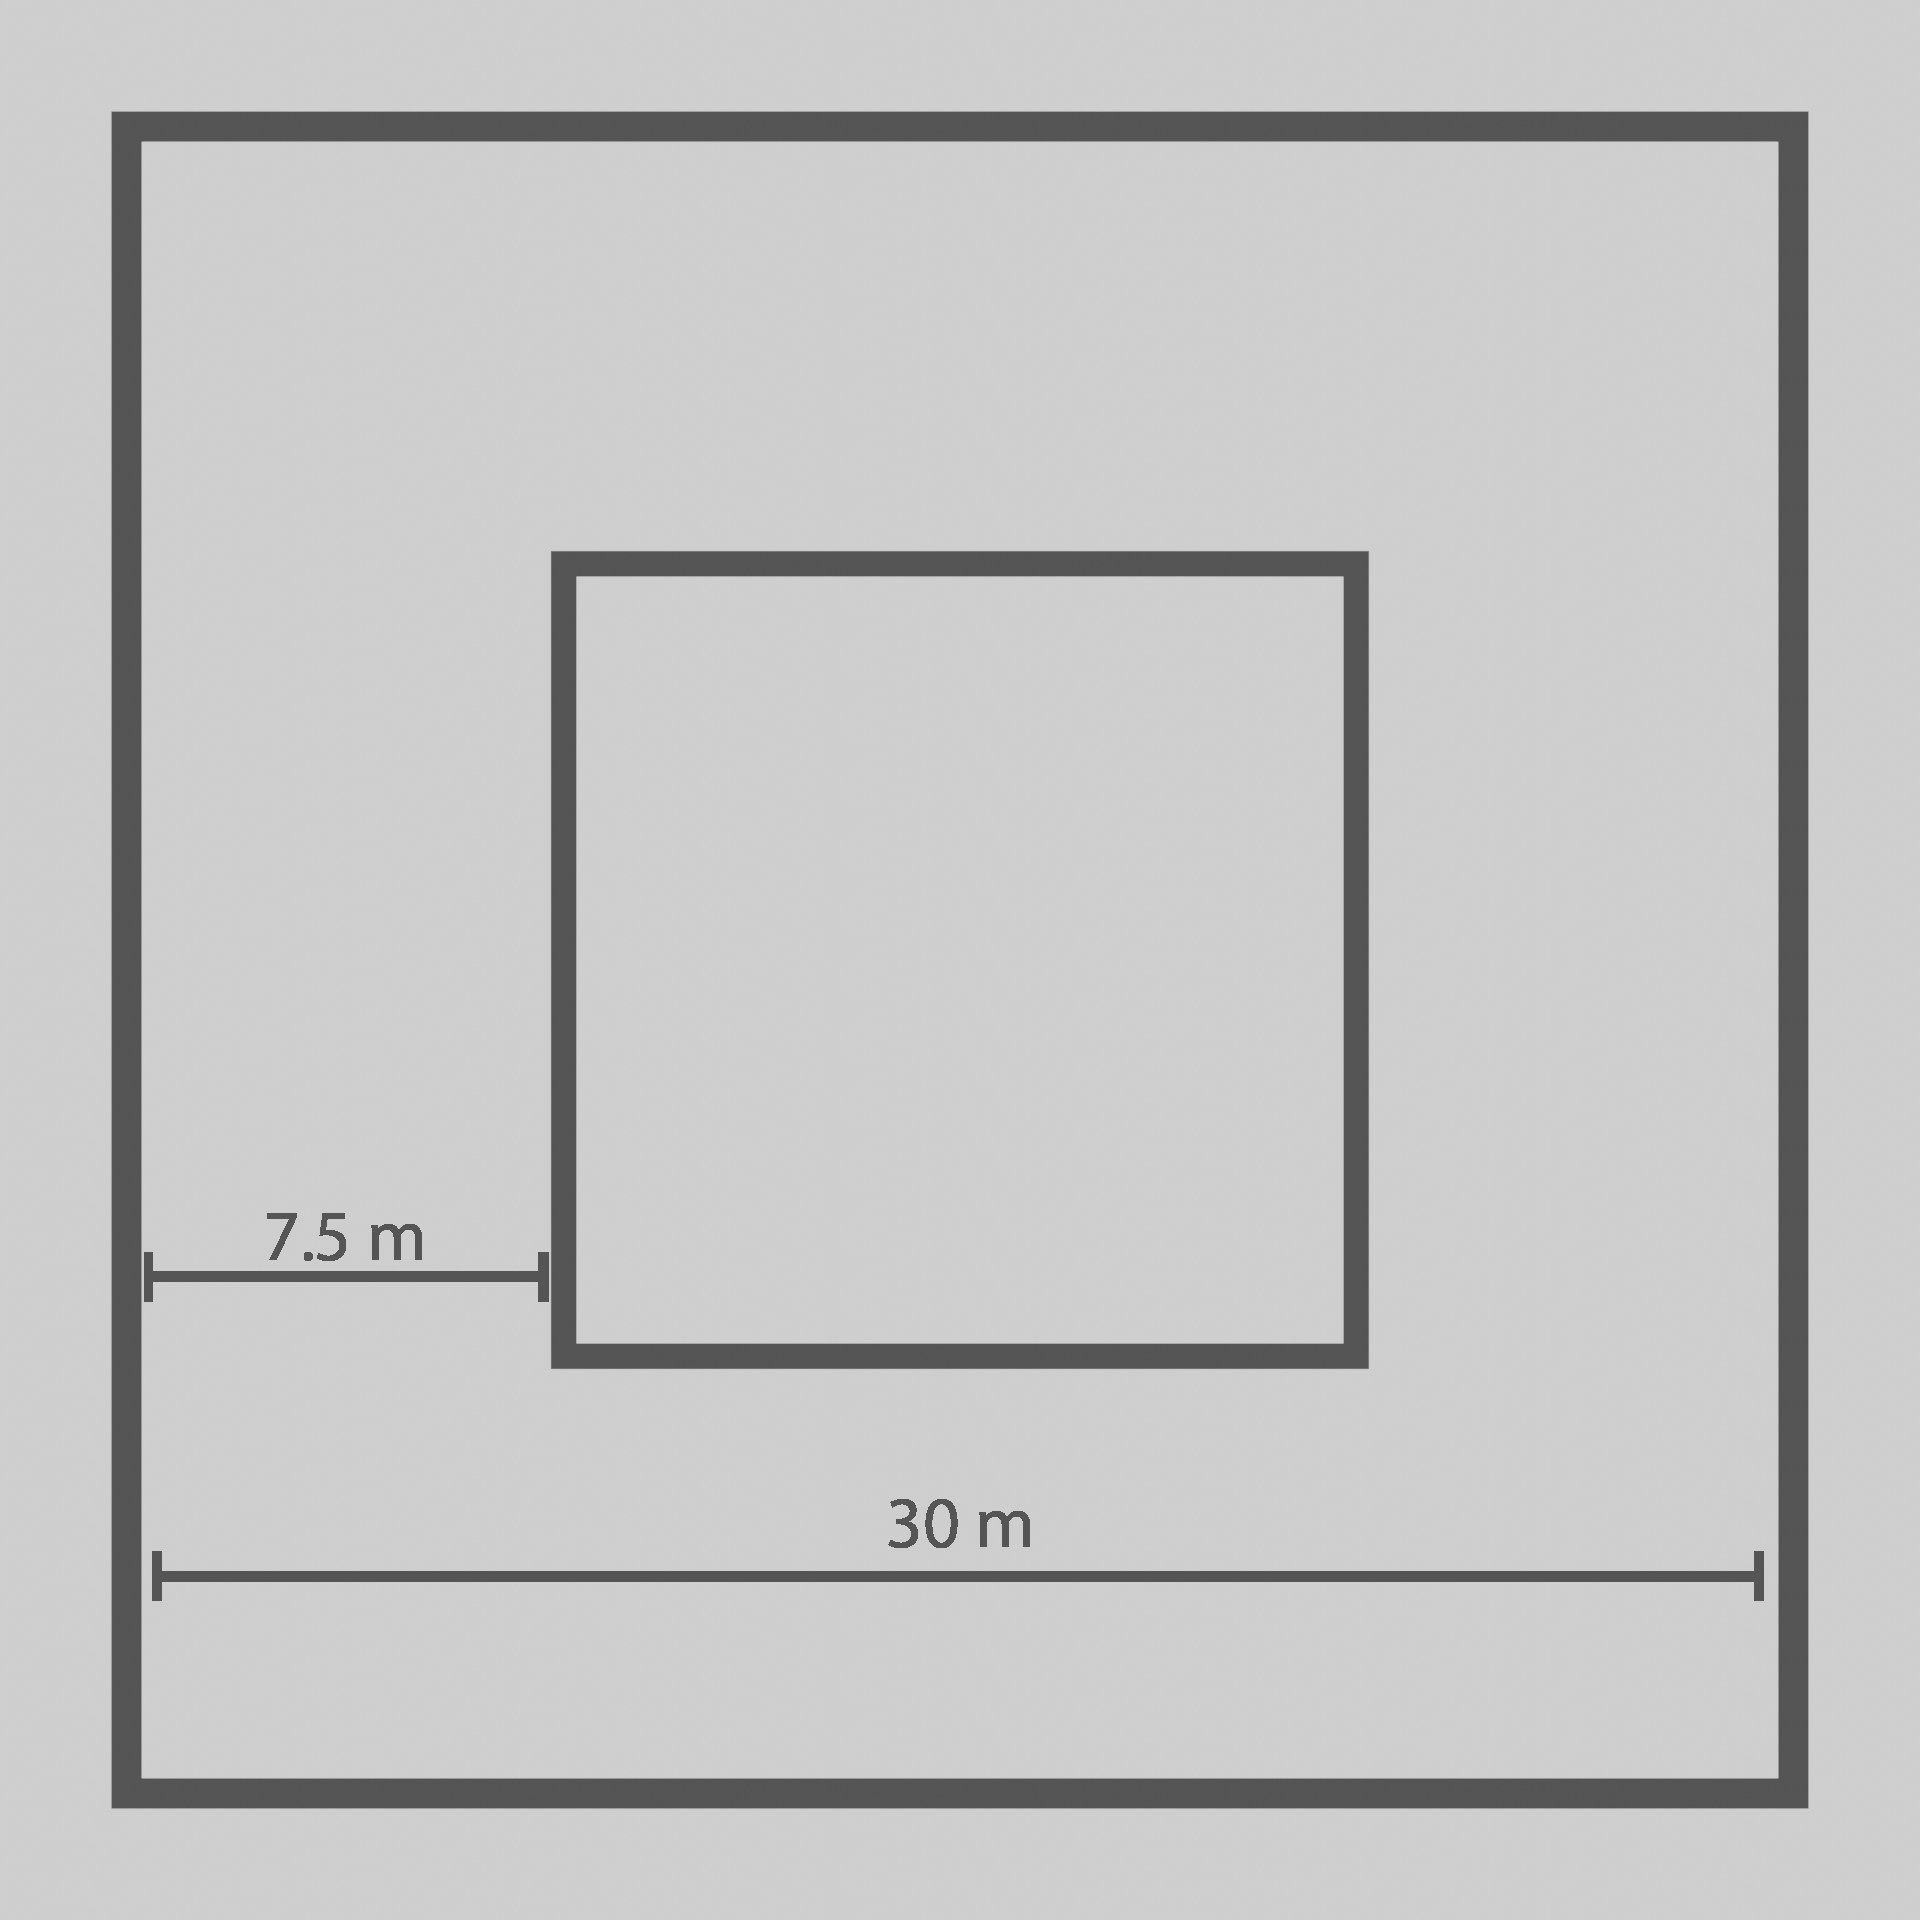
\includegraphics[width=0.45\textwidth]{./Image/Environment/Easy/top_mod.png}
		\vspace{5mm}
		\caption{Simple track images. On the left there is the perspective view and on the right the orthogonal top view with its measurements.}
	\end{figure}
	}\fi
	During training the track is run clockwise and counterclockwise so that the agent learns to turn right and left.
	
	\subsubsection{Complex Track}
	This complex track is used for testing. This will have more long straightaways or sharp turns.
	\ifnum\value{debug}=0 {
	\begin{figure}[H]
    		\centering
\includegraphics[width=0.45\textwidth]{./Image/Environment/Med/perspective.png}
    		%\centering
\includegraphics[width=0.45\textwidth]{./Image/Environment/Med/top.png}	
			\centering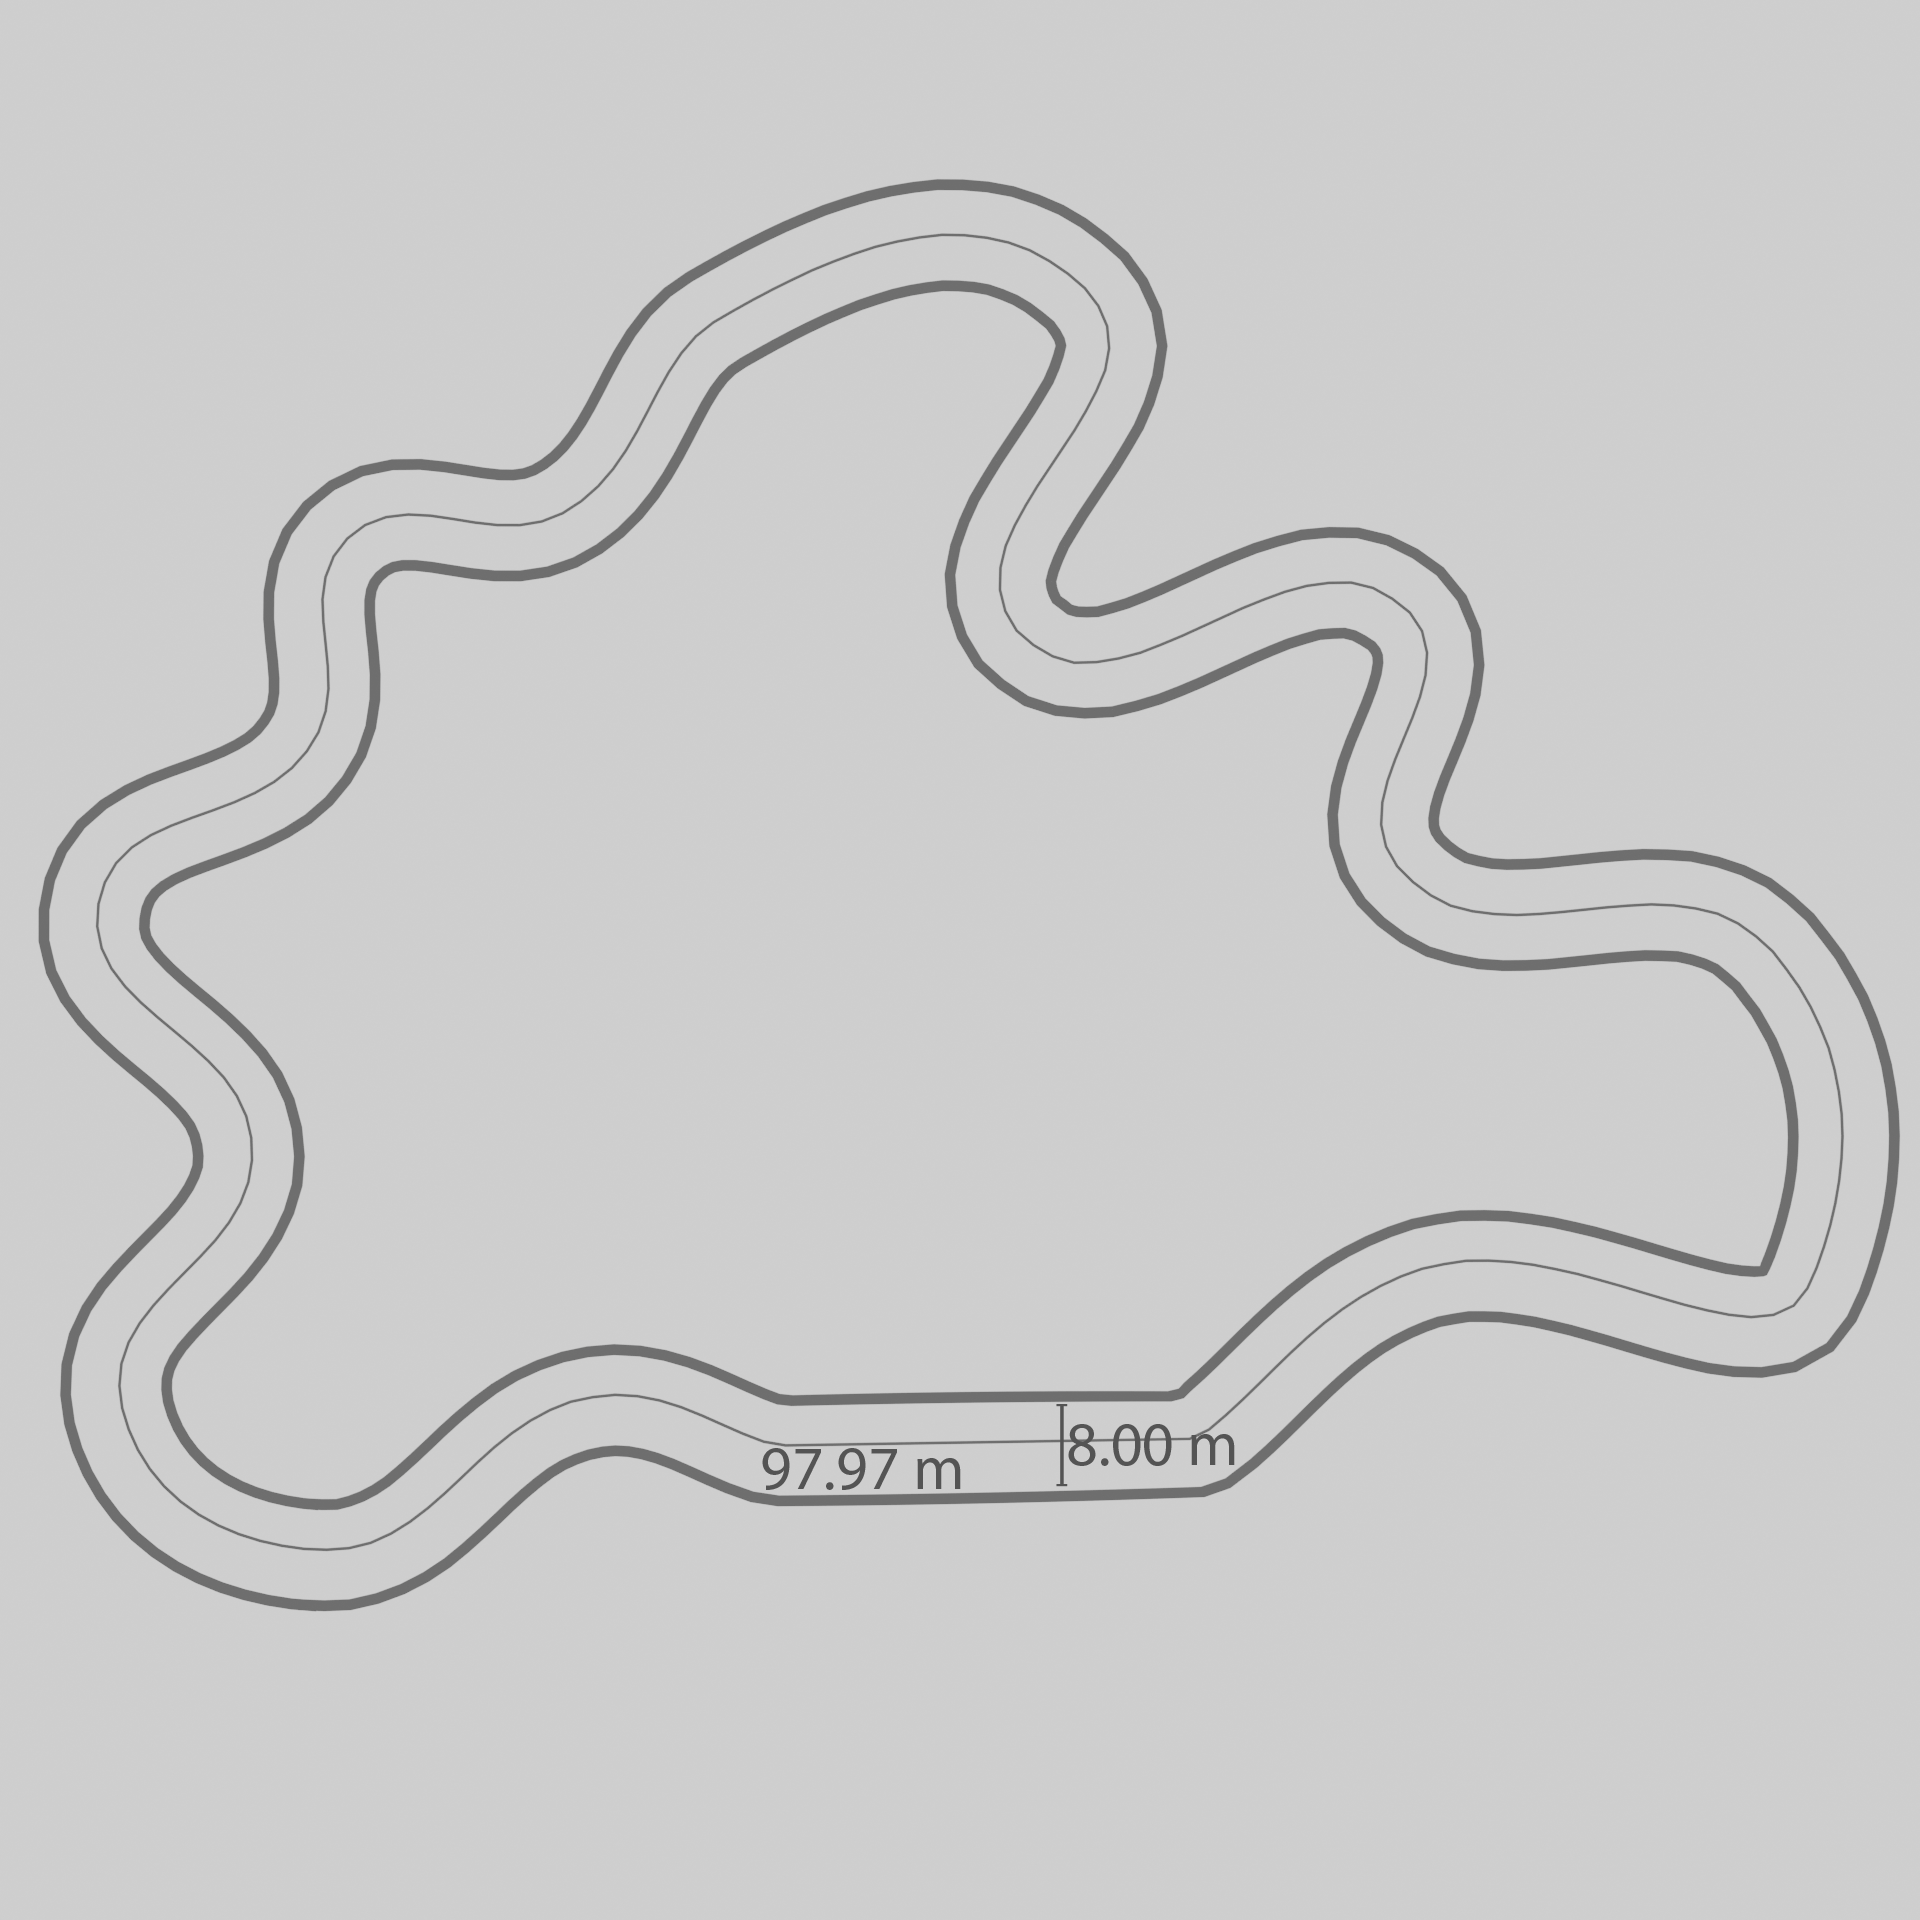
\includegraphics[width=0.45\textwidth]{./Image/Environment/Med/top_w_line_mod.png}
    		
		\vspace{5mm}
		\caption{Complex track images. On the left there is the perspective view and on the right the orthogonal top view with its measurements.}
	\end{figure}
	}\fi
	
	\subsection{Agent}
	\sp
	The agent is a car available on the Vehicle Variety pack \cite{VVp} asset of Unreal Engine 4. From this packet only the `SportCar' content is used and some settings are modified (drag coefficient and other physical values).
	\begin{figure}[H]
    		\centering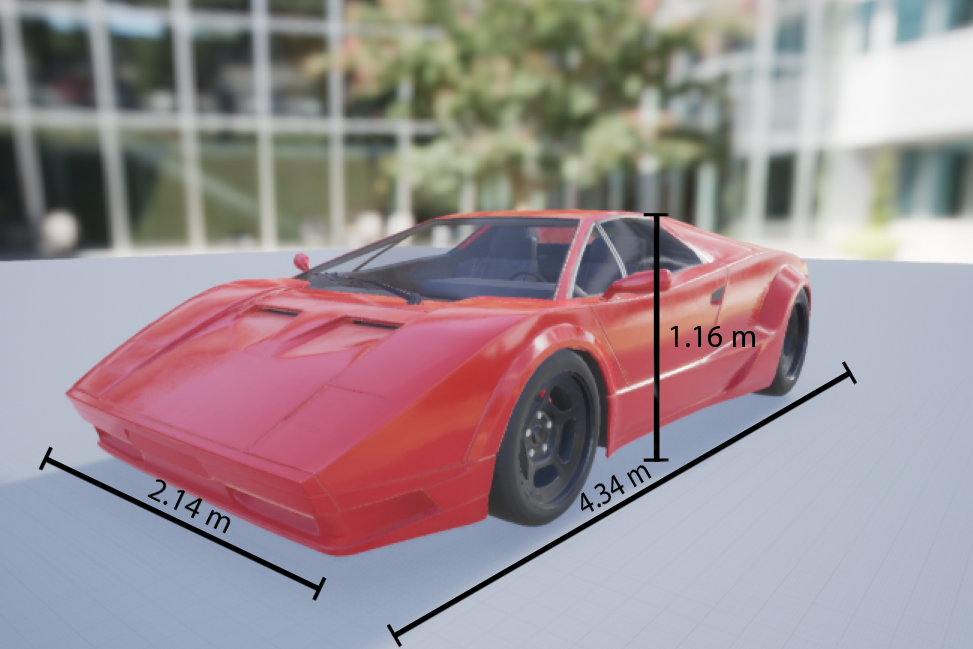
\includegraphics[width=0.9\textwidth]{./Image/Agent/car.png}
		\vspace{2mm}
    		\caption{The used car as Agent with its own measurements.}
	\end{figure}
	
	\subsection{State}
	\sp
	The agent senses the environment around it using some Light Detection and Ranging sensors (\textbf{LiDAR} \cite{LiDAR}). \\
	The number of LiDAR sensors to use is an important hyper-parameter: in this case good results were found using 32 LiDAR sensors. These 32 sensors are equally spaced in an angle range of $170^{\circ}$, this is another important hyper-parameter. \\
	Multiple tests were made to set these hyper-parameters, in particular:
	\begin{itemize}
	\item Too many LiDAR sensors required more training time, they increased the performance but sometimes the model did not converge.
	\item With too few LiDAR sensors the algorithm did not have enough information to learn properly.
	\item Too wide angle decreased the sensor density and decreased the focus on the most important part: the front and the sides of the car.
	\item Too small angle increased the sensor density and increased the focus only on some specific region: the front.
	\end{itemize}
	So a trade-off between training time and performances were reached with 32 sensors and a $170^{\circ}$ angle
	\ifnum\value{debug}=0 {
	\begin{figure}[H] \label{carState}
    		\centering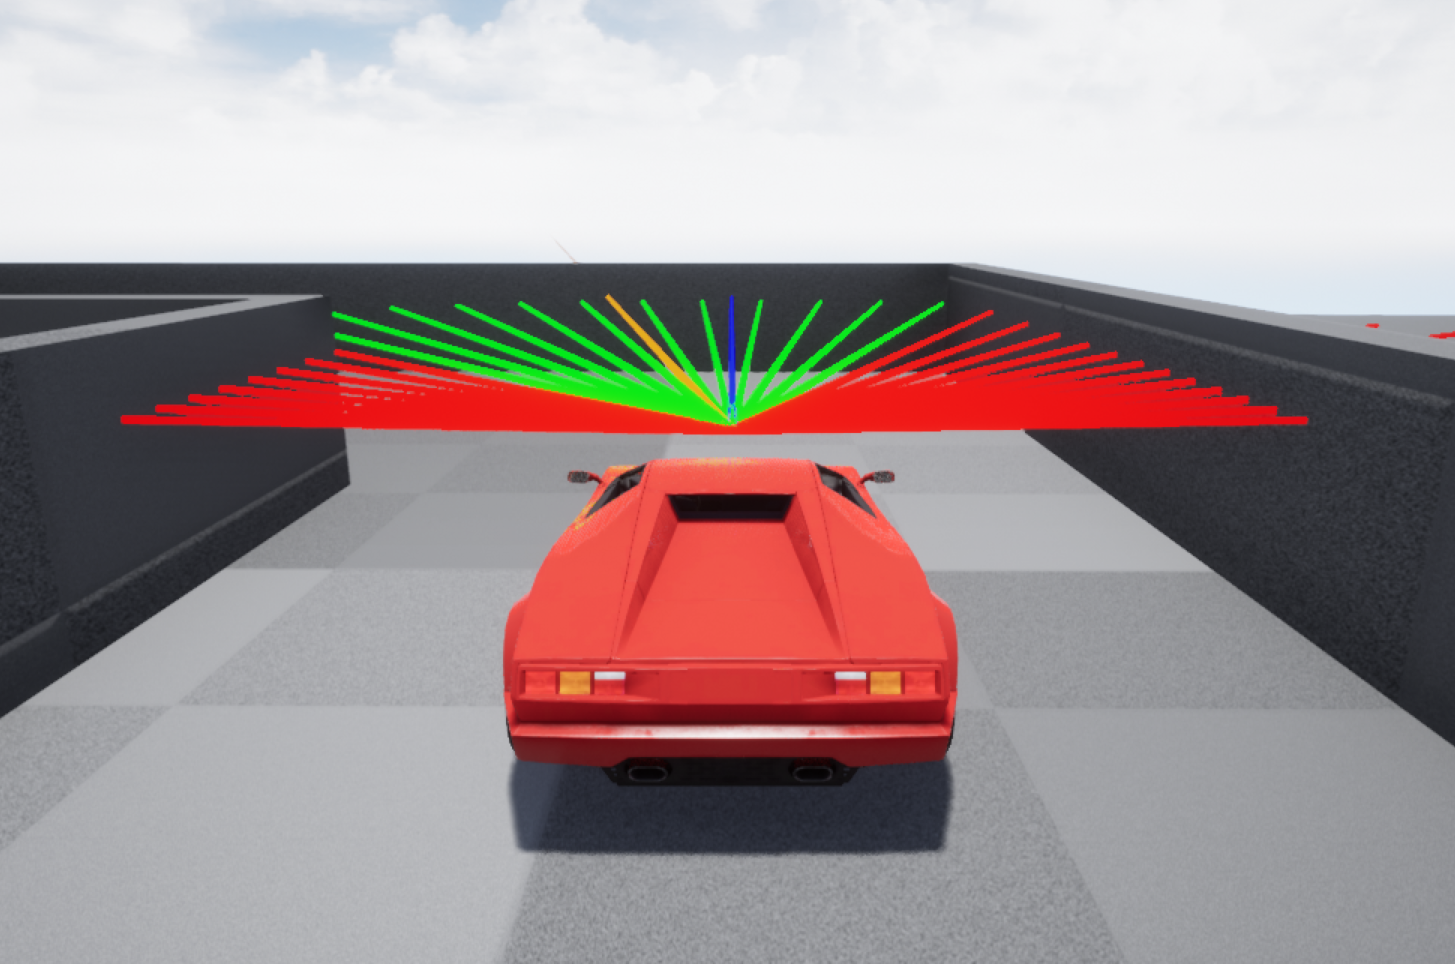
\includegraphics[width=0.9\textwidth]{./Image/State/carSensors.png}
		\vspace{2mm}
		\caption{The image shows how the agent senses the world around it. It is possible to see the $32$ beams equally spaced on a $170^{\circ}$ angle range. \\
		The beam's colour depends on whether the ray has hit an obstacle or not: red object is near enough, green no hit. \\
		There are also two other beams (yellow and blue) they have for visual purposes, in particular to make humans understand how the agent learns; these will be used in the Reward Function \ref{rewardfuc}.}
	\end{figure}
	}\fi
	
	
	\subsection{Policy}
	\sp
	The policy, as mentioned early, is a mapping from state to action: how the agent chooses an action in a given state. The goal is to improve the policy over time in order to increase the cumulative reward. 
	\pp	
	As is common in Reinforcement Learning, the agent needs to explore the environment to get to know the world around it and after some time then apply this knowledge.  This is known as the \textbf{exploration-exploitation trade-off}: at the beginning the agent chooses random actions (exploration), after it has learnt it uses what it knows to choose the correct action (exploitation). \pp
	This exploration-exploitation trade-off is implemented with a value $\epsilon$ initialized to $1$: at each step a random value $c$ (with $c \in [0,1]$) is drawn: if $c\leq\epsilon$ then the agent chooses a random action and $\epsilon$ is decreased otherwise it selects the action $a^\prime$ with the maximum Q-value given the current state $s$ ($\text{max}_{a^\prime}Q_{\theta}(s,a^\prime)$).
	\pp
	The value of $\epsilon$ is decreased with a value $epsilon\_decay = 8.2 \cdot 10^{-5}$; once $\epsilon$ keep decreasing the probability that $c\leq\epsilon$ will be lower so the actor will prefer exploitation over exploration. This is known as \textbf{Epsilon greedy strategy}.\\
	The $epsilon\_decay$ is a hyper-parameter: the lower $epsilon\_decay$ is the more the agent will explore the environment increasing the training time. 
	\pp
	The performance of the policy depends on the neural network structure. In this project 3 different architectures are tested. %The idea behind them is similar, what changes is how the next target Q-value is calculated.; so basically the Bellman equation changes.
	
	\subsubsection{Deep Q-Network}
	\sp
	As mentioned early Deep Q-networks use a neural network to calculate the Q-values given a state and they use \ref{eq:2} to calculate the next Q-value; in particular the target value is calculated with formula \ref{eq:target}, here reported:
	\[
\text{target}_t = r_t + \gamma\text{max}_{a}Q_{\theta}(s_{t+1},a)
\]
and the loss:
\[\mathbb{E}_{(s_t,a_t,r_t,s_{t+1})}[(Q_{\theta}(s_t,a_t) - \text{target}_t)^2]\] 

\tikzset{%
  every neuron/.style={
    circle,
    draw,
    minimum size=1cm
  },
  neuron missing/.style={
    draw=none, 
    scale=4,
    text height=0.333cm,
    execute at begin node=\color{black}$\vdots$
  },
}

\begin{figure}[H]
\begin{center}
	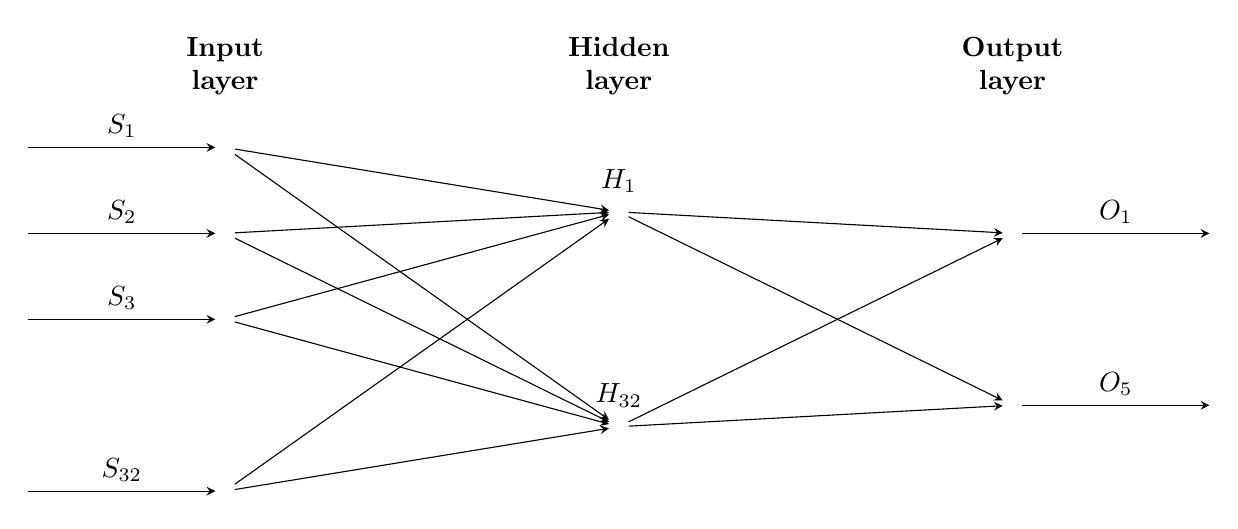
\begin{tikzpicture}[x=25mm, y=0.09\textwidth, >=stealth]
	
	\foreach \m/\l [count=\y] in {1,2,3,missing,4}
	  \node [every neuron/.try, neuron \m/.try] (input-\m) at (0,2.5-\y) {};
	
	\foreach \m [count=\y] in {1,missing,2}
	  \node [every neuron/.try, neuron \m/.try ] (hidden-\m) at (2,2-\y*1.25) {};
	
	\foreach \m [count=\y] in {1,missing,2}
	  \node [every neuron/.try, neuron \m/.try ] (output-\m) at (4,1.5-\y) {};
	
	\foreach \l [count=\i] in {1,2,3,32}
	  \draw [<-] (input-\i) -- ++(-1,0)
	    node [above, midway] {$S_{\l}$};
	
	\foreach \l [count=\i] in {1,32}
	  \node [above] at (hidden-\i.north) {$H_{\l}$};
	
	\foreach \l [count=\i] in {1,5}
	  \draw [->] (output-\i) -- ++(1,0)
	    node [above, midway] {$O_{\l}$};
	
	\foreach \i in {1,...,4}
	  \foreach \j in {1,...,2}
	    \draw [->] (input-\i) -- (hidden-\j);
	
	\foreach \i in {1,...,2}
	  \foreach \j in {1,...,2}
	    \draw [->] (hidden-\i) -- (output-\j);
	
	\foreach \l [count=\x from 0] in {Input, Hidden, Output}
	  \node [align=center, above] at (\x*2,2) {\textbf{\l} \\ \textbf{layer}};
	
	\end{tikzpicture}
	    		\caption{The architecture of the Deep Q-network}
\end{center}
\end{figure}

	One possible problem with this implementation is that both the current Q-value, $Q_{\theta}(s_t,a_t)$, and the next best Q-value, $\text{max}_{a}Q_{\theta}(s_{t+1},a)$, are calculated using the same network, $Q_{\theta}$. This can bring to overestimations of the values, resulting in an over-optimistic value estimate \cite{DDQN1}. 
		
	One possible solution is to use a Double Deep Q-network.
	
	\subsubsection{Double Deep Q-Network} \label{DDQN}
	\sp
	In Double Deep Q-learning 2 networks are used: $Q_{\theta}$ (policy network) and $Q_{\theta^{-}}$ (target network). The 2 networks have the same structure and the weights are initialized with the same values using, in this case, a RandomNormal kernel initializer. \\
	In this case target and loss are calculated as follow:

\[\text{target}_t = r_t + \gamma\text{max}_{a}Q_{\theta^{-}}(s_{t+1},a)\]
\[\mathbb{E}_{(s_t,a_t,r_t,s_{t+1})}[(Q_{\theta}(s_t,a_t) - \text{target}_t)^2]\] 

With this solution current Q-value, $Q_{\theta}(s_t,a_t)$, and the next best Q-value, $\text{max}_{a}Q_{\theta^{-}}(s_{t+1},a)$, are calculated using the 2 different networks ($Q_{\theta}$ and $Q_{\theta^{-}}$). This reduces the bias and increases the score.
\\
Over time the loss between $Q_{\theta}$ and $Q_{\theta^{-}}$ is minimized. The weights of network $Q_{\theta}$ are updated every step using the gradient descent formula while the target network's weights ($Q_{\theta^{-}}$) are update every N steps using \textbf{Polyak averaging}: 
%Value if tau
%https://greentec.github.io/reinforcement-learning-third-en/#soft-update-target-network
\begin{equation} \label{eq:updateweights}
 \theta^{-} = \tau\theta + (1-\tau)\theta^{-} 
 \end{equation}
This is a soft averaging (an hard averaging would be $\theta^{-}=\theta$) weighted by the value $\tau$ (tau). $\tau$ represents how much information it has to be kept from the policy network ($\tau=1$ only the information of the policy network, $\tau=0$ only the information of the target network is keep, no update in this case) \cite{DDQN1,DDQN2}. \\
The value of $\tau$ is usually quite small so that the target network will move slightly to the value of Q-network. Since the value of $tau$ is small, the update should be frequent so that the effect will be noticeable.
\pp
Both N and $\tau$ are hyper-parameters, in this project they are $N=64$ and $\tau=0.001$
\begin{figure}[H]
\begin{center}
	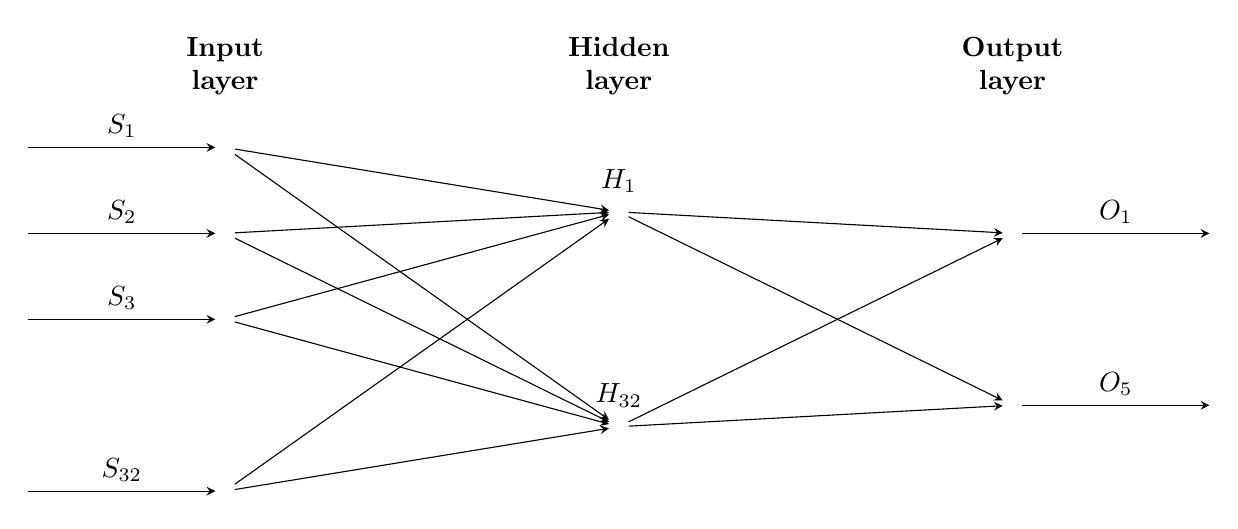
\begin{tikzpicture}[x=25mm, y=0.09\textwidth, >=stealth]
	
	\foreach \m/\l [count=\y] in {1,2,3,missing,4}
	  \node [every neuron/.try, neuron \m/.try] (input-\m) at (0,2.5-\y) {};
	
	\foreach \m [count=\y] in {1,missing,2}
	  \node [every neuron/.try, neuron \m/.try ] (hidden-\m) at (2,2-\y*1.25) {};
	
	\foreach \m [count=\y] in {1,missing,2}
	  \node [every neuron/.try, neuron \m/.try ] (output-\m) at (4,1.5-\y) {};
	
	\foreach \l [count=\i] in {1,2,3,32}
	  \draw [<-] (input-\i) -- ++(-1,0)
	    node [above, midway] {$S_{\l}$};
	
	\foreach \l [count=\i] in {1,32}
	  \node [above] at (hidden-\i.north) {$H_{\l}$};
	
	\foreach \l [count=\i] in {1,5}
	  \draw [->] (output-\i) -- ++(1,0)
	    node [above, midway] {$O_{\l}$};
	
	\foreach \i in {1,...,4}
	  \foreach \j in {1,...,2}
	    \draw [->] (input-\i) -- (hidden-\j);
	
	\foreach \i in {1,...,2}
	  \foreach \j in {1,...,2}
	    \draw [->] (hidden-\i) -- (output-\j);
	
	\foreach \l [count=\x from 0] in {Input, Hidden, Output}
	  \node [align=center, above] at (\x*2,2) {\textbf{\l} \\ \textbf{layer}};
	
	\end{tikzpicture}
	    		\caption{The architecture of the Double Deep Q-network, same as the Deep Q-network. The target network architecture is omitted since identical to this architecture.}
\end{center}
\end{figure}

	\subsubsection{Duelling Double Deep Q-Network}
	%http://proceedings.mlr.press/v48/wangf16.pdf
	\sp
	The Q-value Q(s,a) tells how good it is to take an action a being at state s. This Q-value can be decomposed as the sum of $V(s)$, the value of being at that state, and $A(s,a)$, the advantage of taking that action at the state (from all other possible actions). Mathematically, we can write this as:
	\[ Q(s,a) = V(s) + A(s,a)\]
Duelling Deep Q-network uses two separate estimators for these two components which are then combined together through a special aggregation layer to get an estimate of Q(s,a). By decoupling the estimation, intuitively the Duelling DQN can learn which states are (or are not) valuable without having to learn the effect of each action at each state. This is particularly useful for states where actions do not affect the environment in a meaningful way. \cite{DDQN2} %In these cases, it is unnecessary to evaluate each action for such states and could be skipped to speed up the learning process.
	
The key insight behind this architecture is that for many states, it is unnecessary to estimate the value of each action choice. For example, in the Enduro game setting \cite{Enduro}, knowing whether to move left or right only matters when a collision is imminent. In some states, it is of paramount importance to know which action to take, but in many other states the choice of action has no repercussions on what happens. 
%For bootstrapping based algorithms, however, the estimation of state values is of great importance for every state 
\cite{DDDQN1}. 

With this implementation, the Q-value estimate can be obtained by aggregation:
\begin{equation} \label{eq:DDDQN}
 Q(s,a) = V_{\beta}(s) + A_{\alpha}(s,a) - \frac{1}{|A|} \sum_{a^{\prime}}{A_{\alpha}(s,a^{\prime})}
\end{equation}
where $\beta$ and $\alpha$ are the weights for the $V(s)$ and $A(s,a)$ networks respectively; the subtraction of the advantages of all the actions is used to increase the stability of the optimization.\\
	Training of the duelling architectures, as with standard Deep Q-networks, requires only back-propagation. The estimates $V(s)$ and $A(s,a)$ are computed automatically without any extra supervision or algorithmic modifications. In particular, the Duelling Double Deep Q-network will be used, so there are a policy and a target networks. These networks share the same $N$ and $\tau$ as the Double Deep Q-network \ref{DDQN}
	
\begin{figure}[H]
	\begin{center}
	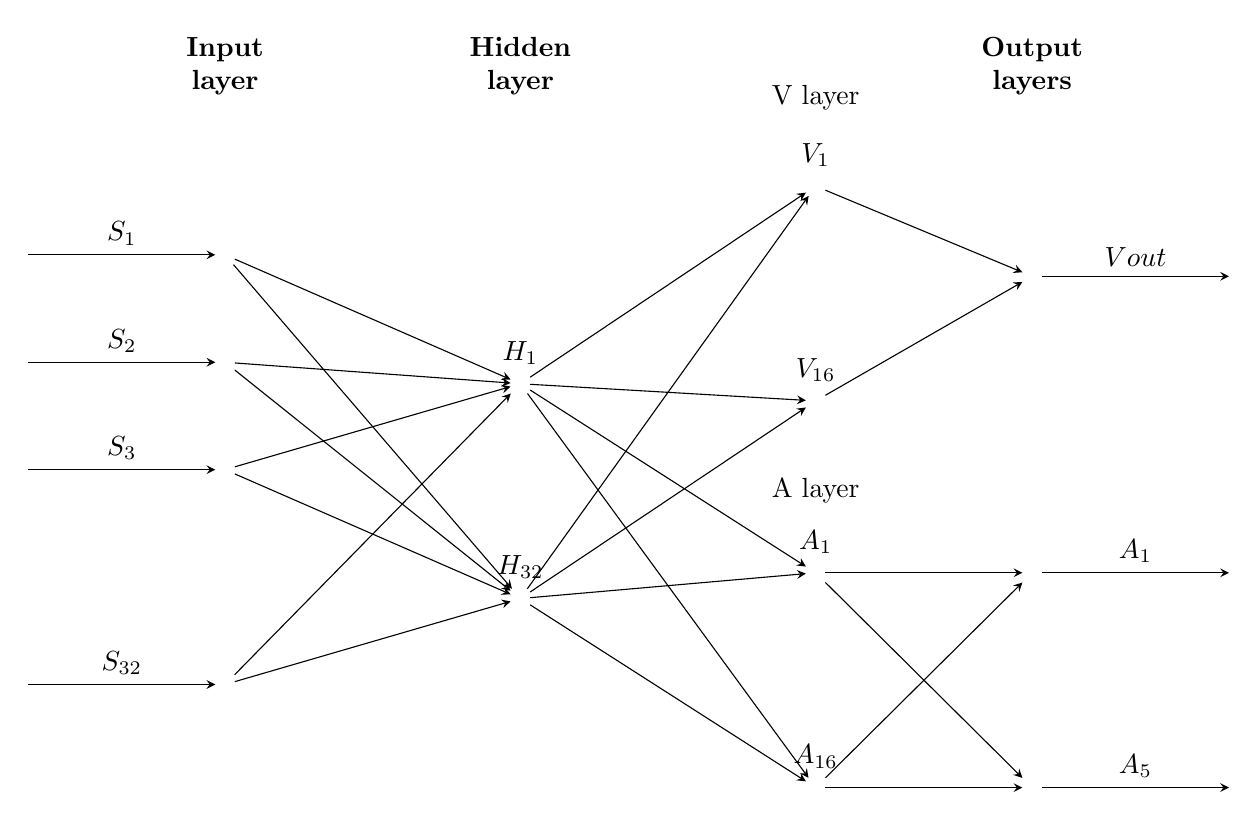
\begin{tikzpicture}[x=25mm, y=0.09\textwidth, >=stealth]
	
	\foreach \m/\l [count=\y] in {1,2,3,missing,4}
	  \node [every neuron/.try, neuron \m/.try] (input-\m) at (0,2.5-\y*1.25) {};
	
	\foreach \m [count=\y] in {1,missing,2}
	  \node [every neuron/.try, neuron \m/.try ] (hidden-\m) at (1.5,1-\y*1.25) {};
	
	%V
	\foreach \m [count=\y] in {1,missing,2}
	  \node [every neuron/.try, neuron \m/.try ] (V-\m) at (3,3.3-\y*1.25) {};
	  
	  \foreach \m [count=\y] in {0}
	  \node [every neuron/.try, neuron \m/.try ] (Vout-\m) at (4.1,1) {};
	  
	  %A
	  \foreach \m [count=\y] in {1,missing,2}
	  \node [every neuron/.try, neuron \m/.try ] (A-\m) at (3,-1.2-\y*1.25) {};
	
	\foreach \m [count=\y] in {1,missing,2}
	  \node [every neuron/.try, neuron \m/.try ] (Aout-\m) at (4.1,-1.2-\y*1.25) {};
	
	
	\foreach \l [count=\i] in {1,2,3,32}
	  \draw [<-] (input-\i) -- ++(-1,0)
	    node [above, midway] {$S_{\l}$};
	    	
	\foreach \l [count=\i] in {1,32}
	  \node [above] at (hidden-\i.north) {$H_{\l}$};
	  
	  %V
	  \foreach \l [count=\i] in {1,16}
	  \node [above] at (V-\i.north) {$V_{\l}$};
	  %A
	  \foreach \l [count=\i] in {1,16}
	  \node [above] at (A-\i.north) {$A_{\l}$};
	
	\foreach \l [count=\i] in {0}
	  \draw [->] (Vout-0) -- ++(1,0)
	    node [above, midway] {$Vout$};
	\foreach \l [count=\i] in {1,5}
	  \draw [->] (Aout-\i) -- ++(1,0)
	    node [above, midway] {$A_\l$};
	
	\foreach \i in {1,...,4}
	  \foreach \j in {1,...,2}
	    \draw [->] (input-\i) -- (hidden-\j);
	
	%V
	\foreach \i in {1,...,2}
	  \foreach \j in {1,...,2}
	    \draw [->] (hidden-\i) -- (V-\j);
	\foreach \i in {1,...,2}
	  \foreach \j in {0}
	    \draw [->] (V-\i) -- (Vout-\j);
	    
%A
	\foreach \i in {1,...,2}
	  \foreach \j in {1,...,2}
	    \draw [->] (hidden-\i) -- (A-\j);
	\foreach \i in {1,...,2}
	  \foreach \j in {1,...,2}
	    \draw [->] (A-\i) -- (Aout-\j);
	
	%\foreach \l [count=\x from 0] in {Input, Hidden, Output}
	%		\node [align=center, above] at (\x*2,2.5) {\l \\ layer};
	  \node [align=center, above] at (0,3) {\textbf{Input} \\ \textbf{layer}};
	  \node [align=center, above] at (1.5,3) {\textbf{Hidden} \\ \textbf{layer}};
	  \node [align=center, above] at (3,2.5) {V layer\\};
	  \node [align=center, above] at (3,-1.75) {A layer};
	  \node [align=center, above] at (4.1,3) {\textbf{Output} \\ \textbf{layers}};	
	\end{tikzpicture}
	\caption{The architecture of the Duelling Double Deep Q-network. The outputs ($V_{out}$ and $A_i$) are then aggregated in formula \ref{eq:DDDQN}.}
\end{center}
\end{figure}


	\subsection{Actions}
	\sp
	There are 2 possible actions the agent is allowed to perform: throttle and steer. These are discretise into 5 actions, from $a_1$ to $a_5$:
	\begin{itemize}
	\item $a_1$, steer to the left:
		\begin{lstlisting}[mathescape=true, language=Python]
		  SetThrottleInput(0.2);
		  SetSteeringInput(-1); \end{lstlisting}
	\item $a_2$, slightly steer to the left:
		\begin{lstlisting}[mathescape=true, language=Python]
		  SetThrottleInput(0.5);
		  SetSteeringInput(-0.5); \end{lstlisting}
	\item $a_3$, go fully forward:
		\begin{lstlisting}[mathescape=true, language=Python]
		  SetThrottleInput(1); \end{lstlisting}
	\item $a_4$, slightly steering to the right:
		\begin{lstlisting}[mathescape=true, language=Python]
		  SetThrottleInput(0.5);
		  SetSteeringInput(0.5); \end{lstlisting}
	\item $a_5$, steer to the right:
		\begin{lstlisting}[mathescape=true, language=Python]
		  SetThrottleInput(0.2);
		  SetSteeringInput(1); \end{lstlisting}
	\end{itemize}
	The values inside the parenthesis are scales to the maximum values (\emph{i.e} SetThrottleInput(-0.5) means that the steering angle il $45*(-0.5)=-22.5^{\circ}$ angle, turn left with the wheels' angle of $22.5^{\circ}$) and they are hyper-parameters.

	
	\subsection{Reward Function} \label{rewardfuc}
	\sp
	Reward function is an important function that tells the agent what is correct and what is wrong using rewards and punishments. \\
	Examples of reward functions can be found in the literature in similar tasks:
	\begin{itemize}
	\item \cite{Paper1} proposes a method where the agent's position and orientation are compared to some ideal values. The desired position is inversely proportional to the distance from the middle of the lane. This reward is maximum equal to 0 when the agent is exactly in the middle of the lane and goes to -1 when reaching a maximum distance from the lane. The desired rotation is inversely proportional to the difference in angle between the agent and the optimal orientation of the trajectory.
	\item In a similar way, \cite{Paper2} proposes a reward function:
	\[
	 r = v cos(\theta)
	\]
	where the reward $r$ is calculated using the speed $v$ of the car and its angle $\theta$ with respect to the road.
	\item other methods employ some checkpoints along the track. Usually these checkpoints are placed manually by humans.
	\end{itemize}
	These methods need some external information, for example where the middle of the road is, where the next checkpoint is and so on.
	\pp 
	The proposed reward function in this project tries only to get information from the car sensors. \\
To explain the reward function an angle $\theta$ must be introduced. This is the angle between the blue ray and orange ray, as shown in figure \ref{carAngle}, where the orange ray is the vectorial sum of all green rays and the blue ray is the car's forward direction.

\ifnum\value{debug}=0 {
\begin{figure}[H] \label{carAngle}
    		\centering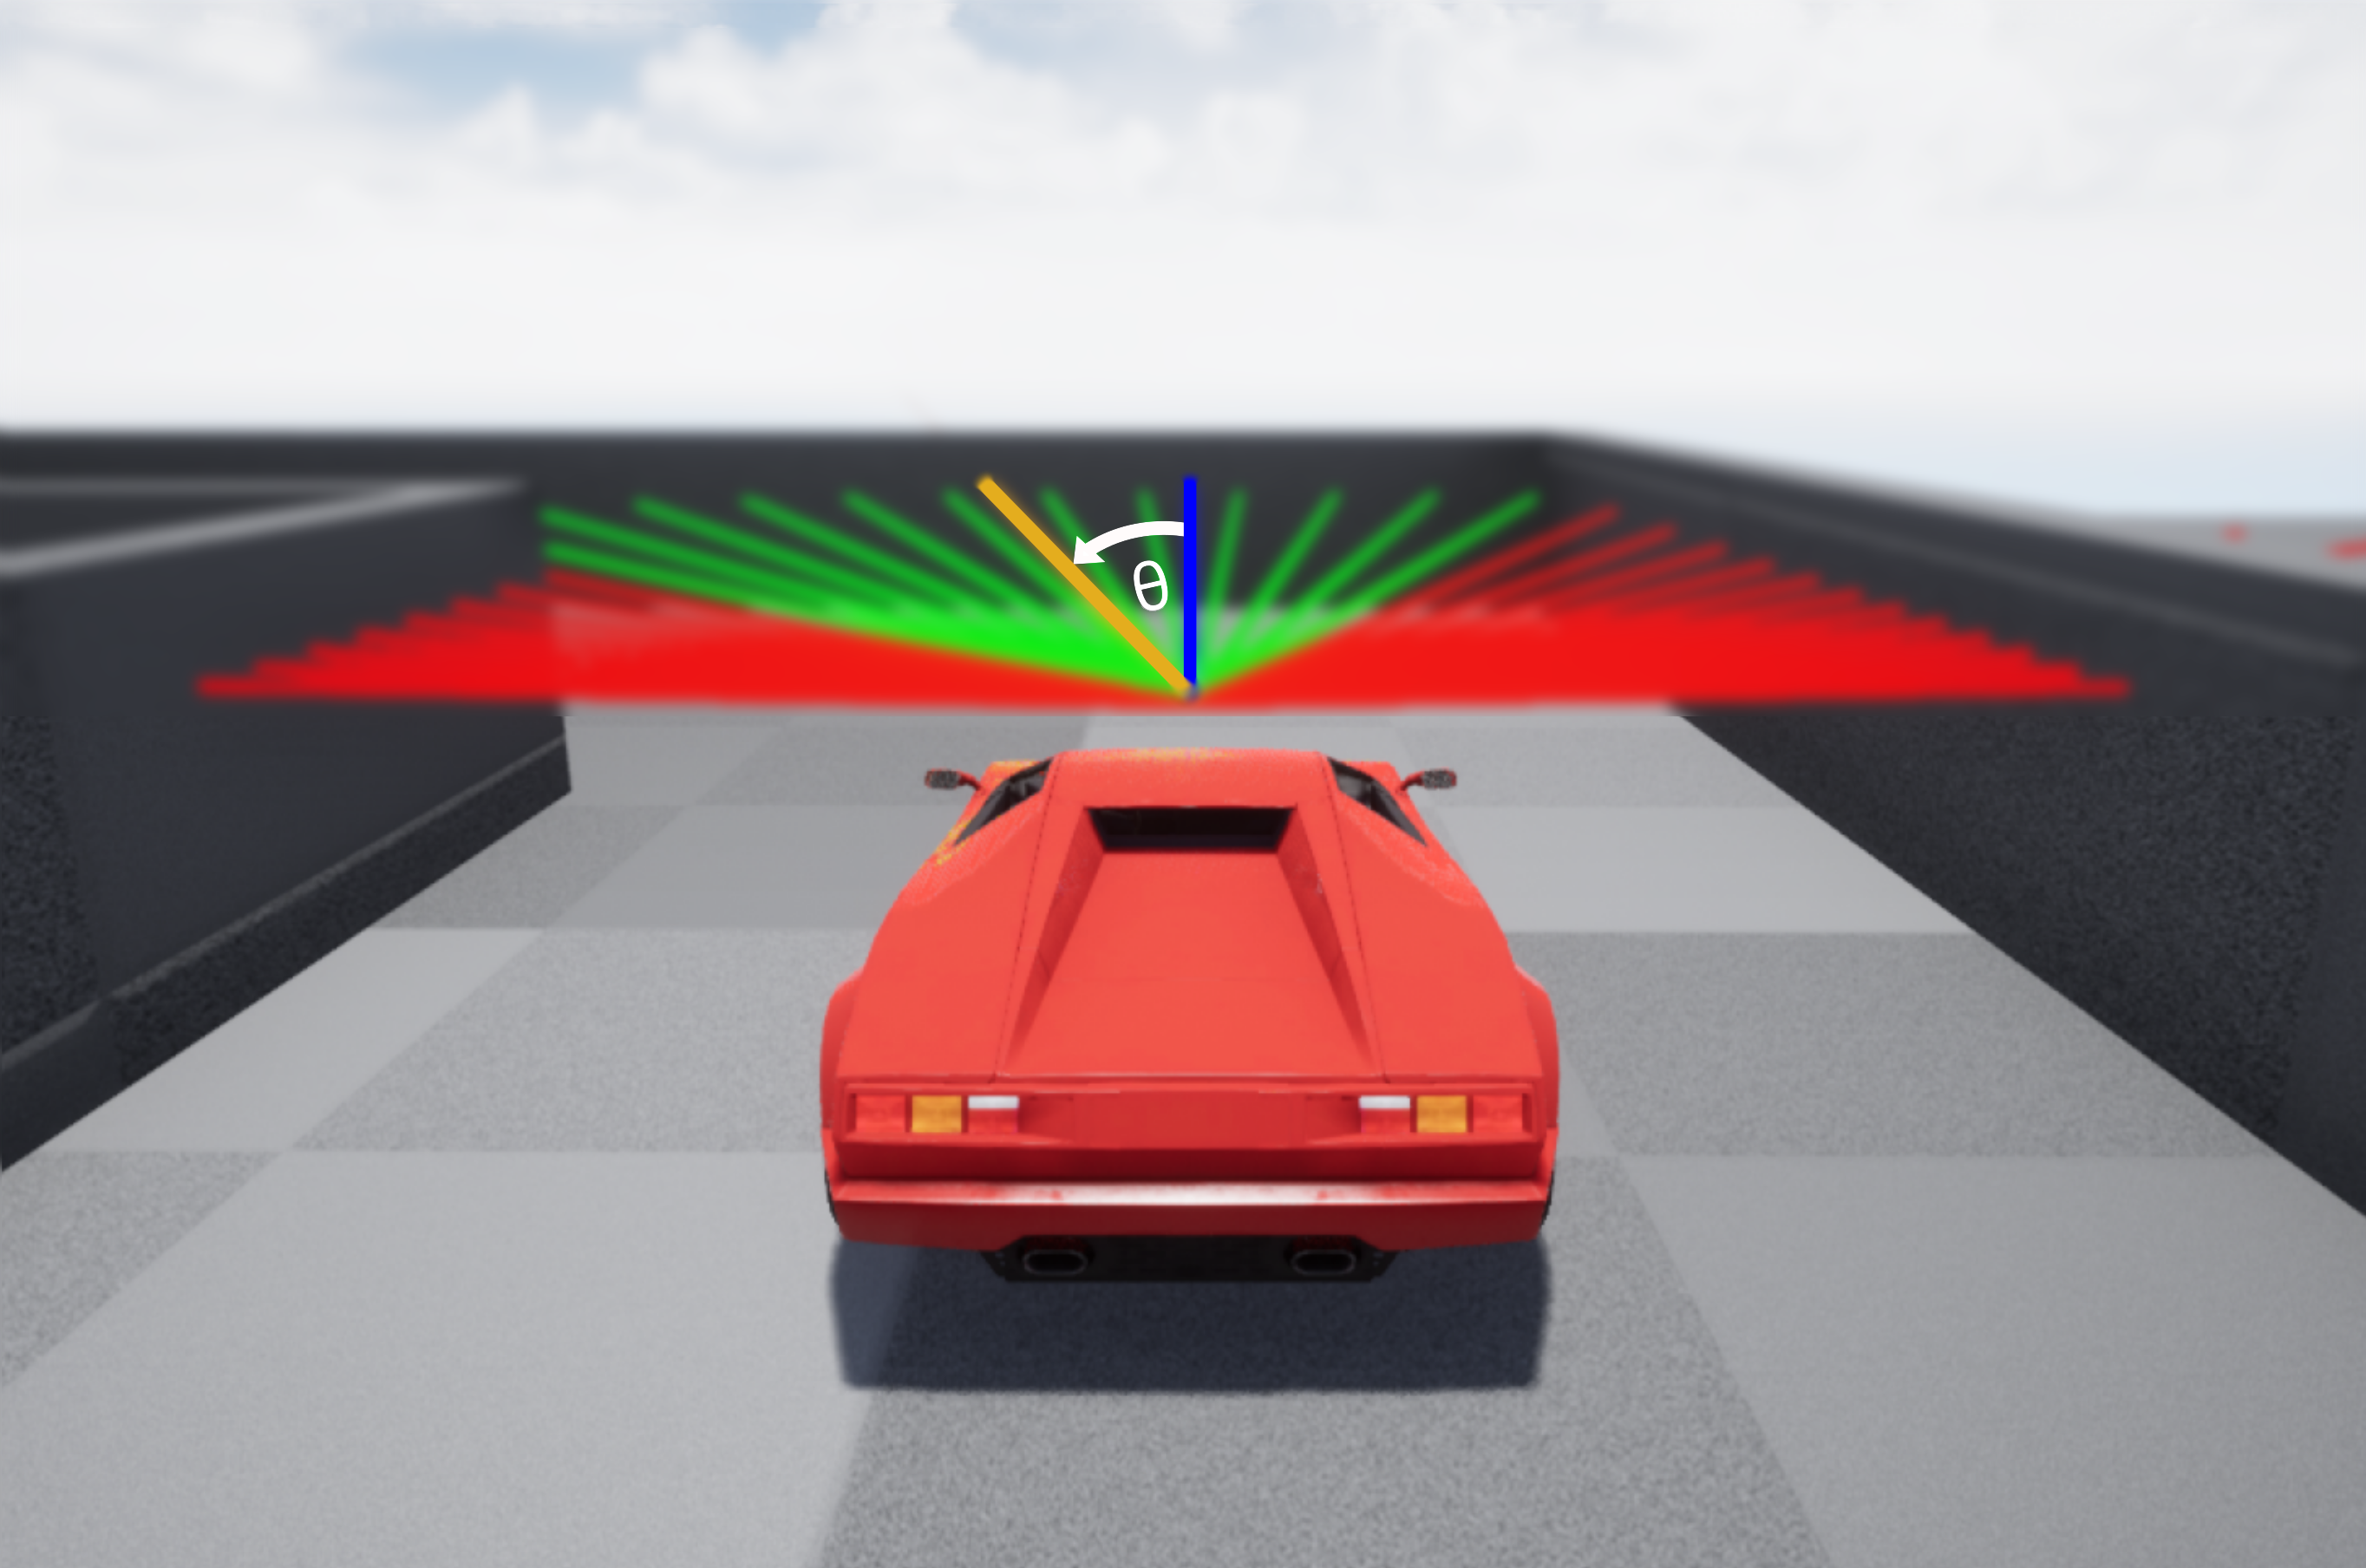
\includegraphics[width=1\textwidth]{./Image/RF/carAngle2.png}
		\vspace{2mm}
    		\caption{The used car as Agent with its own measurements.}
	\end{figure}
} \fi
	Given the angle $\theta$ the reward function is defined as follow:
\begin{lstlisting}[mathescape=true, language=Python]
	if (	($\theta$ > 0 && chosen_action > 2) ||
				($\theta$ < 0 && chosen_action < 2) ||
				(math.abs($\theta$) < forward_angle && chosen_action == 2))
	{
		angle_reward = (number_green_rays - ray_encou_factor) / ray_scal_factor;
	}
	speed_reward = (agent_speed - speed_encou_factor) / speed_scal_factor;
	
	total_reward = angle_reward + speed_reward;
\end{lstlisting}
	Where:
	\begin{itemize}
	\item \emph{chosen\_action} is the action chosen either by exploration or exploitation,
	\item \emph{forward\_angle} is a hyper-parameter (on it depends when the agent should go forward with the max acceleration),
	\item \emph{number\_green\_rays} is the number of green rays (short reminder: the agent can sense the world with rays, these can be visualized as green and red \ref{carState}),
	\item \emph{agent\_speed} is the magnitude of agent's velocity vector, 
	\item \emph{ray\_encou\_factor} and \emph{speed\_encou\_factor} are hyper-parameters and they are encouraging factors, respectively set to $1$ and $250$ (they push the agent to perform better: for example, the factor \emph{speed\_encou\_factor} on the \emph{speed\_reward} means that the agent has to have a speed greater than 250 otherwise the reward is negative; similarly for the \emph{angle\_reward}), 
\item \emph{ray\_scal\_factor} and \emph{speed\_scal\_factor}, set to $10$ and $1000$, are hyper-parameters and they are scaling factors so that the reward is not too large.
\item Finally the \emph{total\_reward} is given by the sum of the 2 rewards.
	\end{itemize}
	
	If the car hits a wall the reward is $-5$.
	
\subsection{Implementation}
\sp
The whole system can be divided in 2 parts: the environment part and the machine learning part:
\begin{itemize}
\item The environment part is developed in Unreal Engine 4 and it includes the environment itself and the physical agent; from this part the agent senses the world, performs actions and gets the rewards.
\item The machine learning part is developed in Python and it is where the neural networks run.
\end{itemize}
The 2 parts communicate through HTTP requests: Unreal Engine is the client and Python is the server. 
\\
The main reason why there are two parts and that they communicate through HTTP requests is that: using Python tools (Tensorflow, etc.) is convenient when dealing with machine learning and write everything in C++ would be time consuming and error proning; Unreal Engine does not allow native communication with Python scripts.
\subsubsection{Client}
\sp
The client starts creating the agent and sending some meta-data (the model to be trained: DQN, DDQN DDDQN, etc.) to the server to initialize it. After the initialization, the run can start with the first episode. An episode has a fixed length of 2000 steps, Unreal Engine updates, but it can end before reaching the 2000 steps if the agent hits an obstacle. An episode start with the positioning of the agent around a point with an offset of the x and y coordinates (this is done to avoid the agent to start always from start same exact point) and with a rotation of $0^{\circ}$ degrees or $180^{\circ}$ degrees so that the agent can circle the track clock or anticlockwise. For each step $t$:
\begin{enumerate}
\item the agent senses the world with LiDAR sensors and obtains the current state $s_t$: an array of 32 values that indicates if for each ray there is an obstacle or not. \label{point1}
\item the agent chooses an action $a_t$, either random or from the neural network. In the former case the epsilon value $\epsilon$ is decreased, with the formula:
\[epsilon = epsilon - epsilon\_decay\]
In the latter case an HTTP request with the current state is sent to the server that will reply with the best action to perform.
\item the agent performs the action chosen gets a reward $r_t$, senses the next state $s_{t+1}$ and evaluate if the next state is an terminal one or not (the agent hits the wall is an terminal state, game over) $g_t$, either 0 or 1.
\item the information of this step is then sent to the server the experience $(s_t,a_t,r_t,s_{t+1},g_t)$.
\item the agent's position is resetted if the terminal state $g_t$ is 1 or the current step number is greater than 2000, otherwise the step number is increased and the loop repeats with point 1.
\end{enumerate}

\subsubsection{Server}
Once the server variables are initialized the server starts waiting for the client's requests. \\
There are 2 main functions: fit and predict.
\begin{itemize}
\item Fit receives an experience as a string from the client and stores it in a list of experiences, query this list to obtain a batch of experiences with which the neural network is trained: the experiences are passed through the network, the best next value is calculated with the neural network (either the policy or target network depending on the model used), the target value is calculated with the Bellman equation. Using the target and the best next value the loss is calculated and then back-propagate through the network to change weights. \\
In the case of DDQN and DDDQN the weights of the target network are updated every N steps using formula \ref{eq:updateweights}.
\item Predict receives a state as string, this is converted to a variable and passed through the network chosen. The prediction is the action which has the maximum Q-value and this is sent back to the client.
\end{itemize}

\end{flushleft}

\newpage
\begin{center}
	\section{Results}
	\sp
\end{center}

\begin{flushleft}
The result shown, for cumulative reward and the average speed, of the 3 models are obtained from 5 different runs: the mean and the confidence intervals are calculated  using the t-distribution (\cite{Tdistri}) with a confidence level of $0.95$. \\
A single run is 150 episodes long and it takes about 50 to 70 minutes.

\subsection{Deep Q-network}
\sp
The result obtained with the Deep Q-network:
\ifnum\value{debug}=0 {
\vspace{-5mm}
	\begin{figure}[H]
    		\centering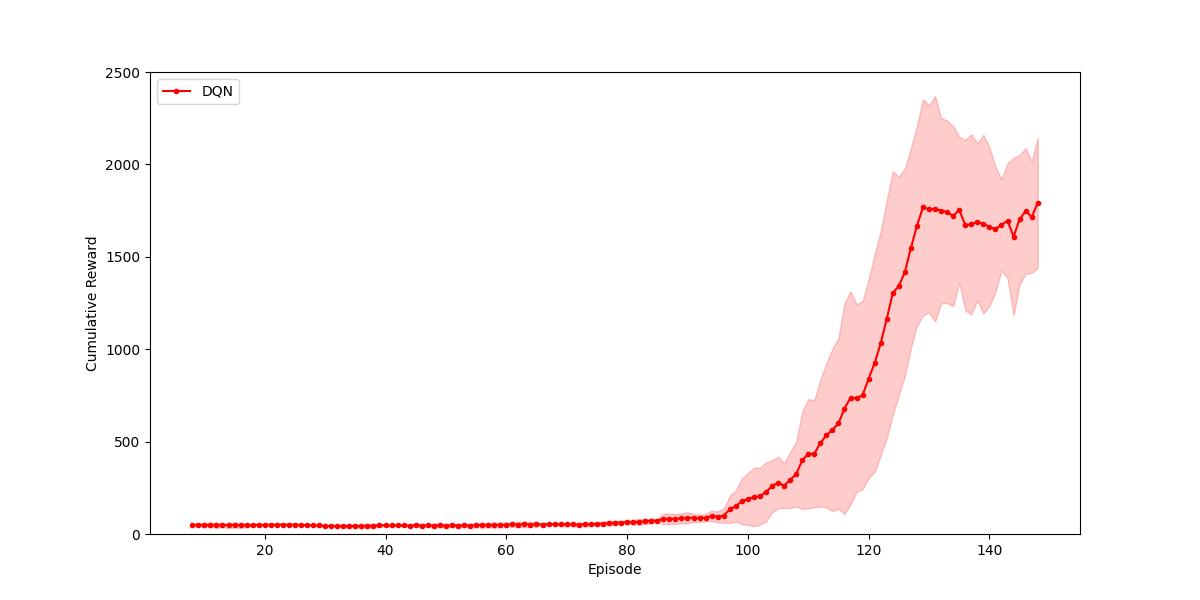
\includegraphics[width=1\textwidth]{./Image/Results/D/plot0_reward.png}
    		\vspace{-5mm}
    		\centering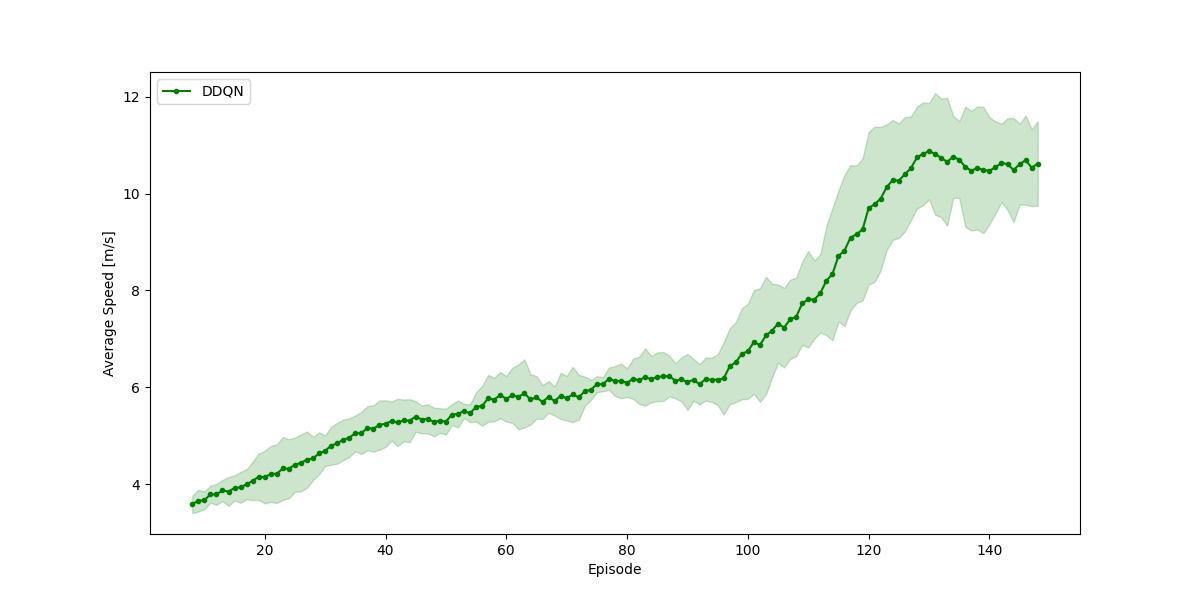
\includegraphics[width=1\textwidth]{./Image/Results/D/plot0_speed.png}
		%\caption{}
	\end{figure}
	}\fi
It is possible to see that the model learnt to drive successfully with not too differences between the runs (the confidence intervals are quite small).
\pp
The plot curves are smothered using an averaging moving window of length 9, this to have more meaningful plots since the focus should be on the trend instead of each single run.

\subsection{Double Deep Q-network}
\sp
The result obtained with the Double Deep Q-network:
\vspace{-5mm}
\ifnum\value{debug}=0 {
	\begin{figure}[H]
    		\centering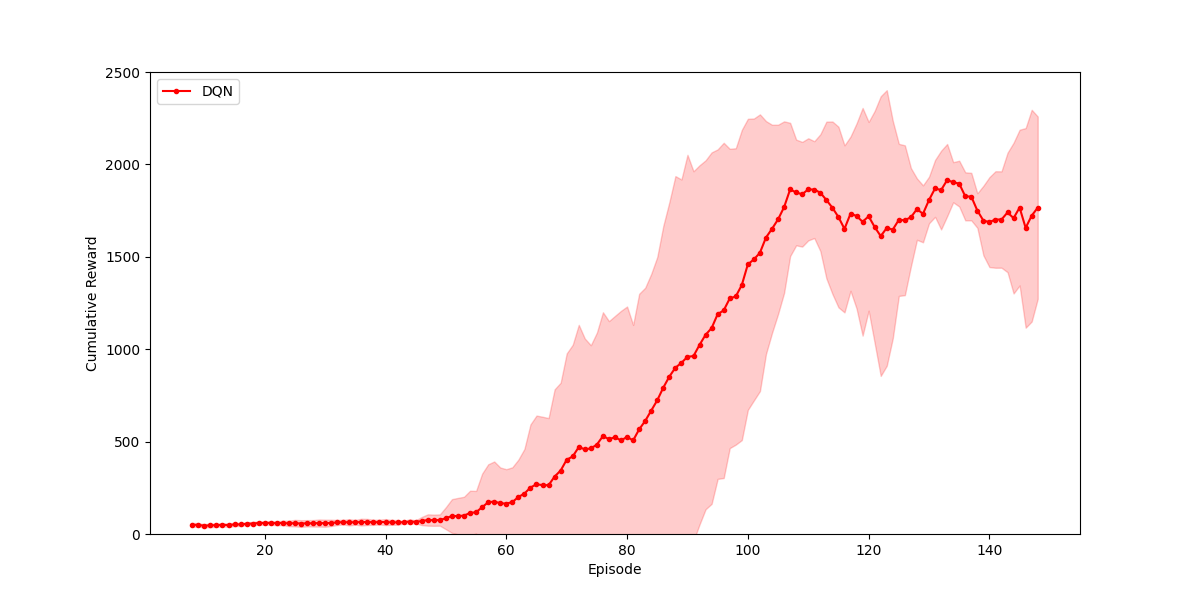
\includegraphics[width=1\textwidth]{./Image/Results/DD/plot1_reward.png}
    		\vspace{-5mm}
    		\centering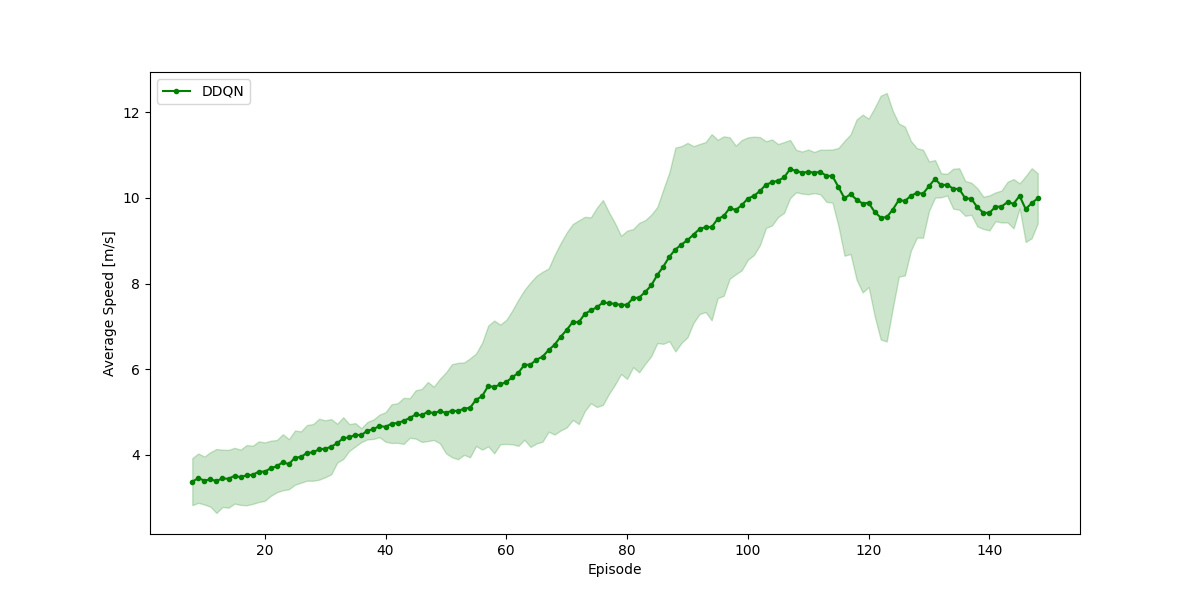
\includegraphics[width=1\textwidth]{./Image/Results/DD/plot1_speed.png}
		%\caption{}
	\end{figure}
	}\fi
	It is possible to see that the model leant to drive successfully with some differences between the runs (the confidence intervals are large).
	
\subsection{Duelling Double Deep Q-network}
\sp
The result obtained with the Duelling Double Deep Q-network:
\vspace{-5mm}
\ifnum\value{debug}=0 {
	\begin{figure}[H]
    		\centering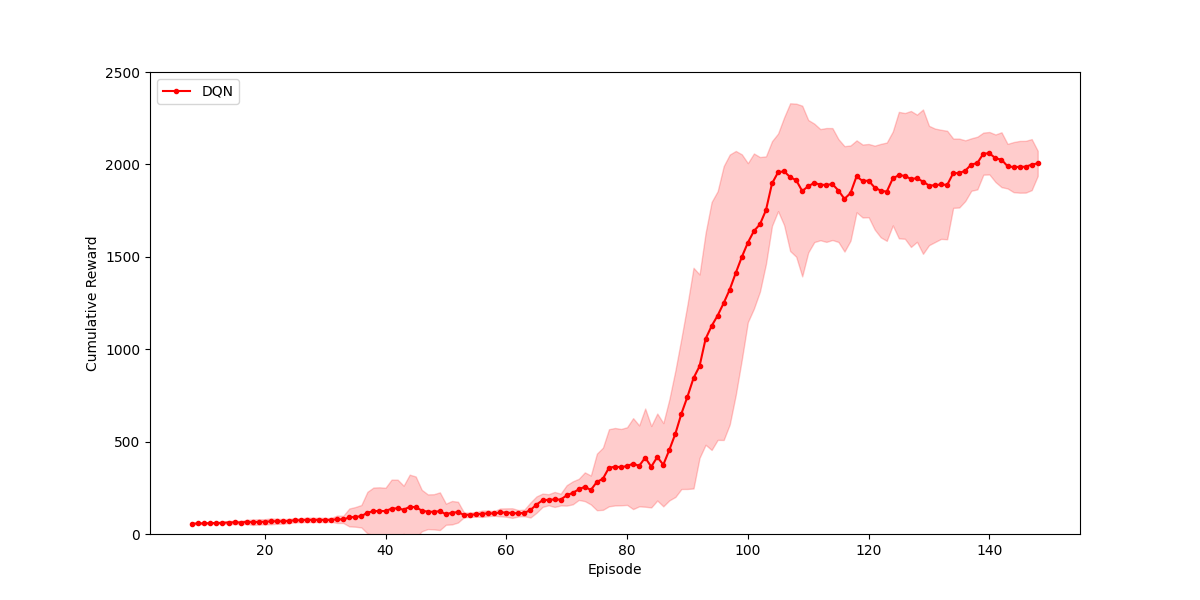
\includegraphics[width=1\textwidth]{./Image/Results/DDD/plot2_reward.png}
    		\vspace{-5mm}
    		\centering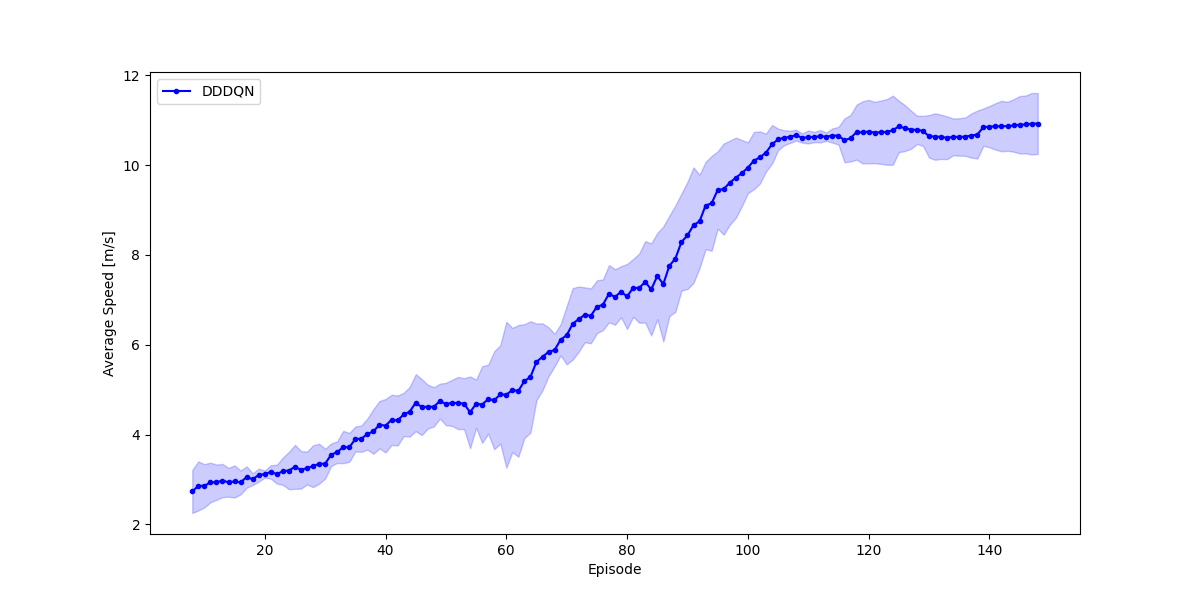
\includegraphics[width=1\textwidth]{./Image/Results/DDD/plot2_speed.png}
		%\caption{}
	\end{figure}
	}\fi
	It is possible to see that the model leant to drive successfully in a stable way (the confidence intervals are small).
	
\subsection{Comparison between models}
\sp
The comparison between the different models:
\ifnum\value{debug}=0 {
	\begin{figure}[H]
    		\centering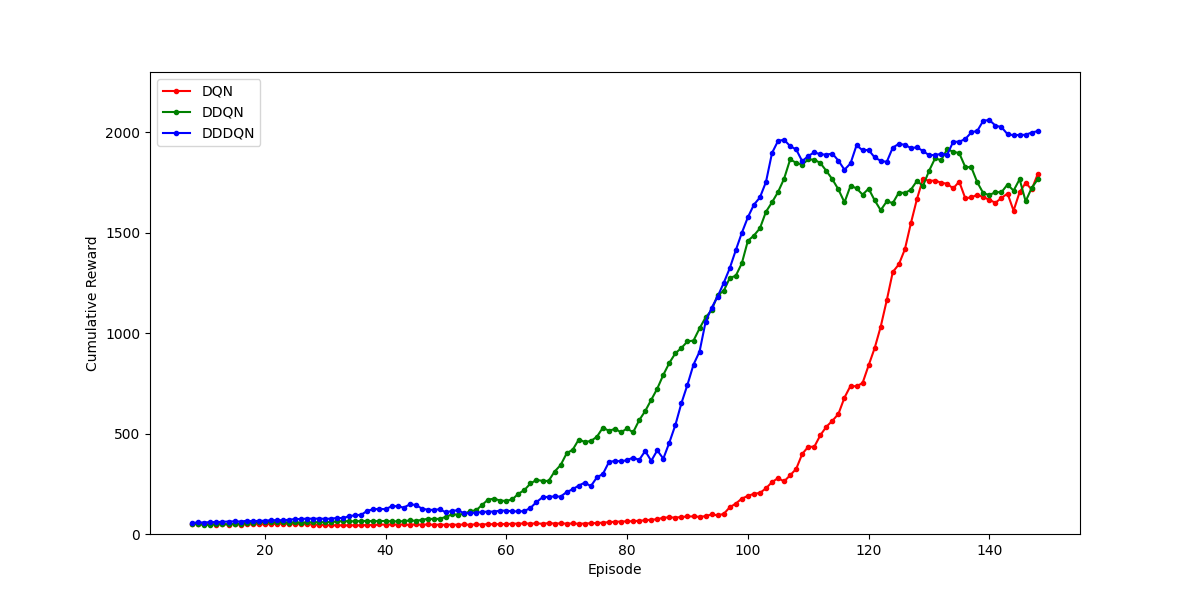
\includegraphics[width=1\textwidth]{./Image/Results/Comparison/rewards.png}
    		\vspace{-5mm}
    		\centering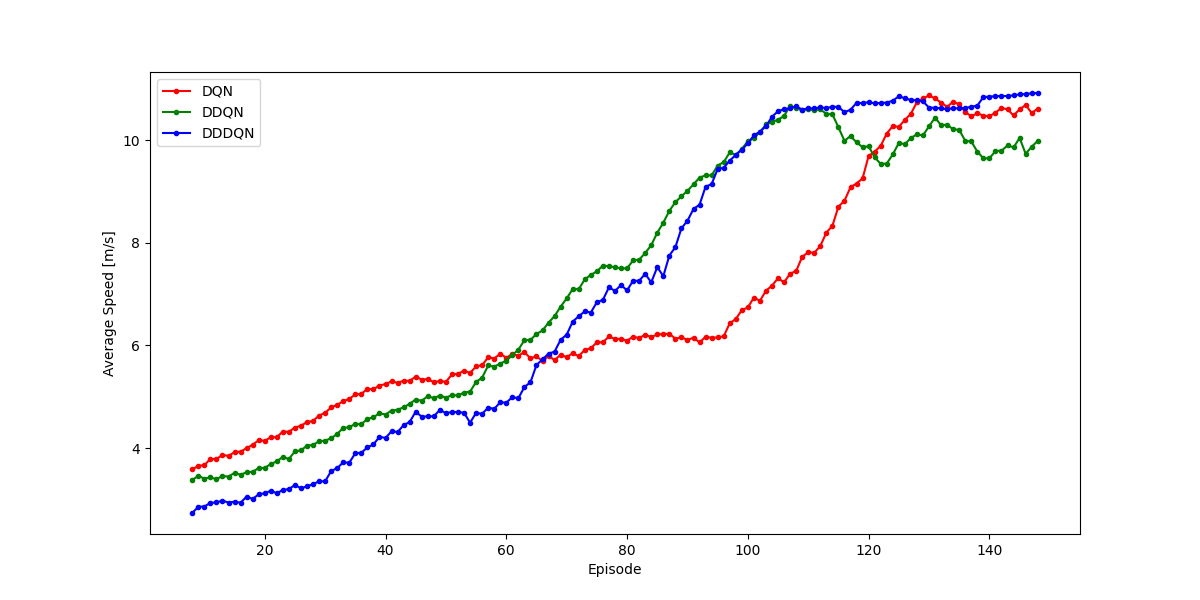
\includegraphics[width=1\textwidth]{./Image/Results/Comparison/speeds.png}
		\caption{Plot of the results of the models. The confidence intervals on these plots are removed to have visually simpler graphs.}
	\end{figure}
	}\fi
	From these plots it is possible to see some differences between the learning paths of the models. In particular:
	\begin{itemize}
	\item The Deep Q-network takes longer to start getting high reward and its peak is less than 2000.
	\item The Double Deep Q-network is fast getting high rewards but it stops at around 2000.
	\item The Duelling Double Deep Q-network is slower than the Double Deep Q-network but it reaches a reward greater than 2000.
	\end{itemize}
	
	\newpage
	\begin{table}[!h]
		\centering
		\resizebox{0.6\textwidth}{!}{%
		\begin{tabular}{|c|c|c|}
		\hline
		\textbf{Model} 	& \textbf{Max Score} & \textbf{Improvement\footnotemark} \\ \hline
		\textbf{DQN}   	&    1791.5                 &    /                   							\\ \hline
		\textbf{DDQN}  &    1915.1                 &   $+6.90\%$                    \\ \hline
		\textbf{DDDQN} &   2060.3                 &  $+7.58\%$                    	\\ \hline
		\end{tabular}
	}
		\caption{Results obtained during the training on the simple track.}
		\label{tab:table-train}
	\end{table}
	\footnotetext{Improvement with respect to the previous model. These are calculated with the following formula: $improvement = (previous\_model\_max - current\_model\_max) / previous\_model\_max * 100$}
	
	
\subsection{Analysis}
\sp
It is possible to see that the model Duelling Double Deep Q-network performs better than the other models this is expected since it is an improvement of the previous models. 
\pp
In particular, the advantage of the duelling architecture lies partly in its ability to learn the state-value function efficiently. Indeed with every update of the Q values in the duelling architecture, the value stream V is updated; this contrasts with the updates in a single-stream architecture where only the value for one of the actions is updated, the values for all other actions remain untouched. This more frequent updating of the value stream in our approach allocates more resources to V and so it allows for better approximation of the state values, which it turns out to be more accurate for temporal difference-based methods like Q-learning \cite{DDDQN1}. \\
This phenomenon is reflected in the experiments .
\pp
An interesting fact is that, the training phase can be divided in 5 periods:
\begin{enumerate}
\item At the beginning the agent does not know anything about the environment and moves randomly, usually hitting a wall in the first steps.
\item After some episodes, the agent starts to learn what action to perform in the different states but it is not confident so the speed is relatively low. It hits a wall after some time, usually because the turns are taken too sharply.
\item Then the agent improves and can confidently finish some laps. The speed increase and the turns are performed with some distance from the walls. Still the agent is not able to reach the 2000 steps.
\item The agent is very good, reaches the maximum speed and it is able to reach the 2000 steps without hitting a wall. It is worth to notice that in this period the agent takes the turns sharply to increase the speed: this was a bad behaviour in period 2 but the agent understands that is the better way to drive to increase the speed and the cumulative reward.
\end{enumerate}

\subsection{Test on Complex Track}
\sp
Results show interesting zero-shot transferability \cite{Zero-shot} of a trained agent in the context of simple track and generalize the knowledge to the complex track. Indeed the simple track is used only for training purposes and the complex track is used for testing purposes (the agent is not trained on the complex track).
\pp
The models are tested on the complex track. The result are here reported:

\ifnum\value{debug}=0 {
	\begin{figure}[H]
    		\centering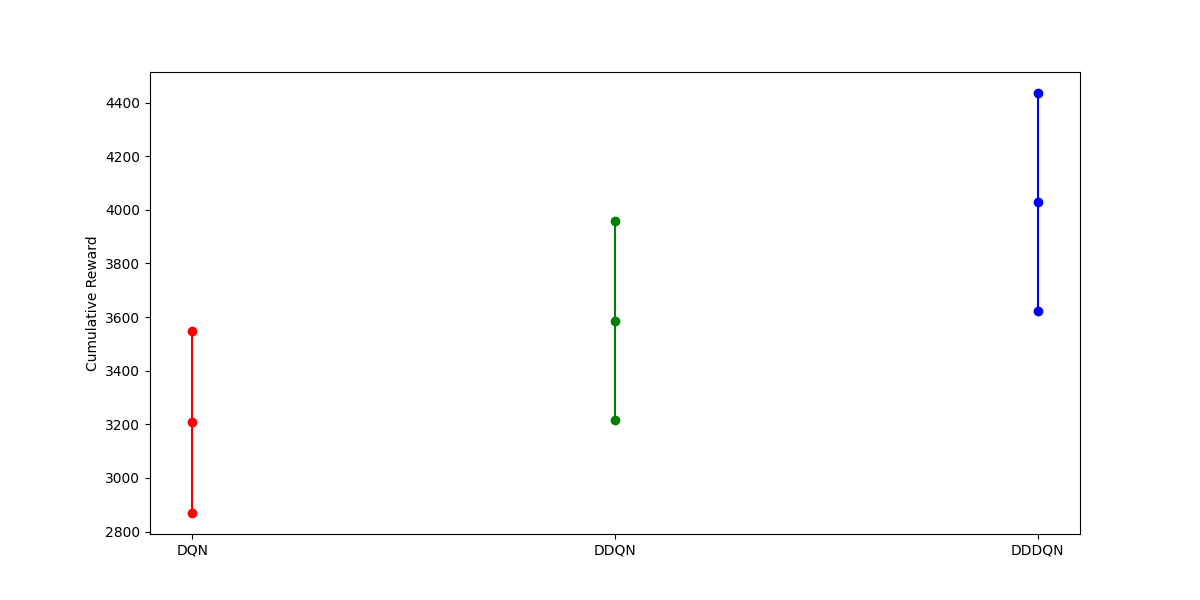
\includegraphics[width=1\textwidth]{./Image/Results/Test/rewards.png}
    		\vspace{-5mm}
    		\centering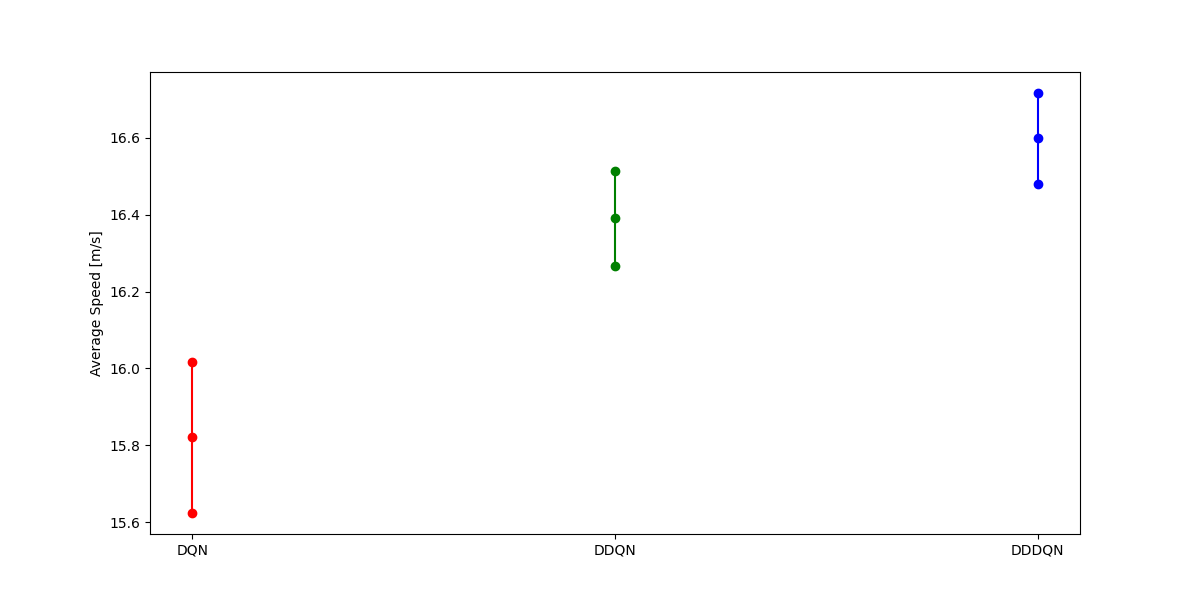
\includegraphics[width=1\textwidth]{./Image/Results/Test/speeds.png}
		\caption{Results of the difference models on the test track. The plots show the average the upper and lower confidence intervals.}
	\end{figure}
	}\fi
	
\begin{table}[H]
		\centering
		\resizebox{0.6\textwidth}{!}{%
		\begin{tabular}{|c|c|c|}
		\hline
		\textbf{Model} 	& \textbf{Avg Score} & \textbf{Improvement\footnotemark} \\ \hline
		\textbf{DQN}   	&    3209.1                 &    /                   							\\ \hline
		\textbf{DDQN}  &    3586.9                 &   $+11.77\%$                    \\ \hline
		\textbf{DDDQN} &   4029.4                 &  $+12.33\%$                    	\\ \hline
		\end{tabular}
	}
		\caption{Result obtained during the evaluation of the models on the complex track.}
		\label{tab:table-test}
	\end{table}
	\footnotetext{Improvement with respect to the previous model. Calculation similar to table \ref{tab:table-train}}
	
	For each model 10 consecutive runs are performed then the results are averaged and the confidence intervals calculated.

\end{flushleft}

\newpage
\begin{center}
	\section{Conclusion}
	\sp
\end{center}
\begin{flushleft}

This project was a formative experience that allowed me to discover many new topics. Moreover, it allowed me to understand that there is a substantial difference between the university environment and the research environment: university, as mentioned by some professors during the courses, has the task of giving a general knowledge of the topics and the real task is to give a way of thinking and analysing a problem to find a solution; indeed, during this project I realized that computer related knowledge was not always essential but it was more important to understand what was needed to be done and how to do it.
\ppn

 I am fully satisfied with the project as an AI researcher and developer. I believe this project was very useful because it allowed me to deepen and to learn about new topics and gave me an idea to understand if the tasks assigned could be addressed in a future university career or in a possible job.
\\
Moreover, this was an experience that allowed me to grow both personally and professionally, not to mention that it is a way to enrich the Curriculum Vitae.

\subsection{Possible future works}
%\sp
To conclude this report, here some possible future ideas that could be addressed in a next experience:
\begin{itemize}
\item find better hyper-parameters, maybe running a grid search even if it would be expensive;
\item perform more runs so that the confidence intervals are smaller;
\item set up an actual robot and then transfer the trained models to the real world and test their performances (check whether the results are the same and model DDDQN is still the best).
\item to use cameras instead of LiDARs to get the agent's state. Similar projects: \cite{Nworks1, Nworks2}
\item Test other Reinforcement Learning models. For example, an interesting model would be the Deep Deterministic Policy Gradient (\textbf{DDPG}) to solve the same task but with a continuous action space \cite{Nworks3}.
\end{itemize}

\end{flushleft}

%References
\newpage
\section{References}
\begingroup
\renewcommand{\section}[2]{}
\begin{thebibliography}{999}
   \bibitem{AVtaxonomy}
  SAE. 2016.
  \emph{Taxonomy and Definitions for Terms Related to Driving Automation Systems for On-Road Motor Vehicles}.\\
  \url{https://www.sae.org/standards/content/j3016_201806/}
   
  \bibitem{AVlevels}
  Monika Stoma, Agnieszka Dudziak, Jacek Caban and Paweł Drozdzie. 2021.
  \emph{The Future of Autonomous Vehicles in the Opinion of Automotive
Market Users}.\\
  \url{https://www.mdpi.com/1996-1073/14/16/4777/pdf}
   
   \bibitem{AVlevels2}
  Piotr CZECH, Katarzyna TUROŃ, Jacek BARCIK. 2018.
  \emph{AUTONOMOUS VEHICLES: BASIC ISSUES}.\\
  \url{https://doi.org/10.20858/sjsutst.2018.100.2}
  
\bibitem{AVfirm}
  Todd Litman. 2021.
  \emph{Autonomous Vehicle Implementation Predictions}.\\
  \url{https://www.vtpi.org/avip.pdf}
  
     \bibitem{AVparking}
  Paul Barter. 2013.
  \emph{"Cars are parked 95\% of the time". Let's check!}.\\
  \url{https://www.reinventingparking.org/2013/02/cars-are-parked-95-of-time-lets-check.html}
  
   \bibitem{AVbenefit}
  Jeremy A. Carp. 2018.
  \emph{AUTONOMOUS VEHICLES: PROBLEMS AND PRINCIPLES FOR FUTURE REGULATION}.\\
  \url{https://scholarship.law.upenn.edu/cgi/viewcontent.cgi?article=1048&context=jlpa}
 
   \bibitem{RLandSL}
  ANDREW G. BARTO and THOMAS G. DIETTERICH.
  \emph{Reinforcement Learning and its Relationship to Supervised Learning}.\\
  \url{http://web.engr.orst.edu/~tgd/publications/Barto-Dietterich-03.pdf}
  
  \bibitem{RLapplications}
  Yuxi Li. 2019.
  \emph{REINFORCEMENT LEARNING APPLICATIONS}.\\
  \url{https://arxiv.org/pdf/1908.06973.pdf}
  
  \bibitem{TDl}
  Scholarpedia.org
  \emph{Temporal difference learning}.\\
  \url{http://www.scholarpedia.org/article/Temporal_difference_learning}
 
  \bibitem{Blender}
  \emph{Blender}.\\
  \url{https://www.blender.org/}
   
     \bibitem{UE4}
  \emph{Unreal Engine 4}.\\
  \url{https://www.unrealengine.com/}
   
   
   \bibitem{VVp}
  \emph{Vehicle Variety Pack}.\\
  \url{https://www.unrealengine.com/marketplace/en-US/product/bbcb90a03f844edbb20c8b89ee16ea32}
  
     \bibitem{LiDAR}
  \emph{LiDAR}.\\
  \url{https://en.wikipedia.org/wiki/LiDAR}
  
  \bibitem{DDQN1}
  Hado van Hasselt and Arthur Guez and David SilverGoogle DeepMind. 2015.
  \emph{Deep Reinforcement Learning with Double Q-learning}.\\
  \url{  https://arxiv.org/pdf/1509.06461.pdf}
   \bibitem{DDQN2}
  Swagat Kumar. 2020.
  \emph{Balancing a CartPole System with Reinforcement Learning}.\\
  \url{https://arxiv.org/pdf/2006.04938v2.pdf}
 
 
  \bibitem{Enduro}
  	Atari 2600. 1983.
  \emph{Enduro (video game)}.\\
  \url{https://en.wikipedia.org/wiki/Enduro_(video_game)}
  \bibitem{DDDQN1}
  	Ziyu Wang, Tom Schaul, Matteo Hessel, Hado van Hasselt, Marc Lanctot, Nando de Freitas. Google DeepMind, London, UK. 2015.
  \emph{Duelling Network Architectures for Deep Reinforcement Learning}.\\
  \url{https://arxiv.org/pdf/1511.06581.pdf}
   
   
   \bibitem{Paper1}
  	Marin Toromanoff, Emilie Wirbel, Fabien Moutarde. 2020.
  \emph{End-to-End Model-Free Reinforcement Learning
for Urban Driving using Implicit Affordances}.\\
  \url{https://openaccess.thecvf.com/content_CVPR_2020/papers/Toromanoff_End-to-End_Model-Free_Reinforcement_Learning_for_Urban_Driving_Using_Implicit_Affordances_CVPR_2020_paper.pdf}

  \bibitem{Paper2}
  	Rohan Chopra and Sanjiban Sekhar Roy. 2020.
  \emph{End-to-End Reinforcement Learning
for Self-driving Car}.\\
  \url{http://eprints.kmu.ac.ir/30207/8/SPRINGER\%20book-compressed.pdf\#page=65}
  
  \bibitem{Tdistri}
  	Wikipedia. Student's t-distribution.
  \emph{Student's t-distribution}.\\
  \url{https://en.wikipedia.org/wiki/Student%27s_t-distribution}
  
  \bibitem{Zero-shot}
  	Daniele Gammelli, Kaidi Yang, James Harrison, Filipe Rodrigues, Francisco C. Pereira, Marco Pavone. 2021.
  \emph{Graph Neural Network Reinforcement Learning for Autonomous Mobility-on-Demand Systems}.\\
  \url{https://arxiv.org/pdf/2104.11434.pdf}
  
  \bibitem{Nworks1}
  	Riku Arakawa, Shintaro Shiba. 2020.
  \emph{Exploration of Reinforcement Learning for Event Camera using
Car-like Robots}.\\
  \url{https://arxiv.org/pdf/2004.00801.pdf}
  \bibitem{Nworks2}
  	Peide Cai, Hengli Wang, Huaiyang Huang, Yuxuan Liu, and Ming Liu. 2021.
  \emph{Vision-Based Autonomous Car Racing Using Deep
Imitative Reinforcement Learning}.\\
  \url{https://arxiv.org/pdf/2107.08325.pdf}
  \bibitem{Nworks3}
  Timothy P. Lillicrap, Jonathan J. Hunt, Alexander Pritzel, Nicolas Heess,
Tom Erez, Yuval Tassa, David Silver and Daan Wierstra. Google Deepmind, 2019.
  \emph{CONTINUOUS CONTROL WITH DEEP REINFORCEMENT
LEARNING}.\\
  \url{https://arxiv.org/pdf/1509.02971.pdf}
  
  
   \bibitem{PaperRef}
  	Shumin Feng, Bijo Sebastian and Pinhas Ben-Tzvi. 2021.
  \emph{A Collision Avoidance Method Based on Deep
Reinforcement Learning}.\\
  \url{https://www.mdpi.com/2218-6581/10/2/73/pdf}

\end{thebibliography}

\end{document}
